\documentclass[a4paper,14pt]{extarticle}

% Путь до папки с общими шаблонами
\newcommand{\pathToCommonFolder}{../../Common}
% Название работы в титуле
\newcommand{\workname}{Отчет по практическим работам}
% Название дисциплины в титуле
\newcommand{\discipline}{Теория автоматов}
% Название кафедры в титуле
\newcommand{\kafedra}{Кафедра Вычислительной техники}
% Тема работы в титуле
\newcommand{\theme}{Сложение чисел с плавающей точкой}
% Должность преподавателя в титуле
\newcommand{\rang}{ассистент}
% ФИО преподавателя в титуле
\newcommand{\teacherfio}{А.~С.~Боронников}


\usepackage{tabularx}

\usepackage{booktabs}
\newcolumntype{b}{X}
\newcolumntype{s}{>{\hsize=.5\hsize}X}
\newcommand{\heading}[1]{\multicolumn{1}{c}{#1}}

\usepackage{extsizes} % Возможность сделать 14-й шрифт

% Вставка заготовки преамбулы
% Этот шаблон документа разработан в 2014 году
% Данилом Фёдоровых (danil@fedorovykh.ru) 
% для использования в курсе 
% <<Документы и презентации в \LaTeX>>, записанном НИУ ВШЭ
% для Coursera.org: http://coursera.org/course/latex .
% Исходная версия шаблона --- 
% https://www.writelatex.com/coursera/latex/5.3

% В этом документе преамбула

% Для корректного использования русских символов в формулах
% пакеты hyperref и настройки, связанные с ним, стоит загуржать
% перед загрузкой пакета mathtext



% поддержка русских букв
% кодировка шрифта
%\usepackage[T2A]{fontenc} 
\usepackage{pscyr}

% использование ненумеровонного абзаца с добавлением его в содержаниеl

\newcommand{\anonsection}[1]{\section*{#1}\addcontentsline{toc}{section}{#1}}
\newcommand{\sectionunderl}[1]{\section*{\underline{#1}}}


% настройка окружения enumerate
\usepackage{enumitem}
\setlist{noitemsep}
\setlist[enumerate]{labelsep=*, leftmargin=1.5pc}

\usepackage{hyperref}

% сначала ставить \usepackage{extsizes} % Возможность сделать 14-й шрифт
% для корректной установки полей вставлять преамбулу следует в последнюю очередь (но перед дерективой замены \rmdefault)
\usepackage[top=20mm,bottom=25mm,left=35mm,right=20mm]{geometry} % Простой способ задавать поля

\hypersetup{				% Гиперссылки
	unicode=true,           % русские буквы в раздела PDF
	pdftitle={Заголовок},   % Заголовок
	pdfauthor={Автор},      % Автор
	pdfsubject={Тема},      % Тема
	pdfcreator={Создатель}, % Создатель
	pdfproducer={Производитель}, % Производитель
	pdfkeywords={keyword1} {key2} {key3}, % Ключевые слова
	colorlinks=true,       	% false: ссылки в рамках; true: цветные ссылки
	linkcolor=red,          % внутренние ссылки
	citecolor=black,        % на библиографию
	filecolor=magenta,      % на файлы
	urlcolor=blue           % на URL
}

%%% Работа с русским языком
\usepackage{cmap}					% поиск в PDF
\usepackage{mathtext} 				% русские буквы в формулах
\usepackage[T2A]{fontenc}			% кодировка
\usepackage[utf8]{inputenc}			% кодировка исходного текста
\usepackage[english,russian]{babel}	% локализация и переносы
\usepackage{indentfirst}
\frenchspacing

%для изменения названия списка иллюстраций
\usepackage{tocloft}


\renewcommand{\epsilon}{\ensuremath{\varepsilon}}
\renewcommand{\phi}{\ensuremath{\varphi}}
\renewcommand{\kappa}{\ensuremath{\varkappa}}
\renewcommand{\le}{\ensuremath{\leqslant}}
\renewcommand{\leq}{\ensuremath{\leqslant}}
\renewcommand{\ge}{\ensuremath{\geqslant}}
\renewcommand{\geq}{\ensuremath{\geqslant}}
\renewcommand{\emptyset}{\varnothing}

% Изменения параметров списка иллюстраций
\renewcommand{\cftfigfont}{Рисунок } % добавляем везде "Рисунок" перед номером
\addto\captionsrussian{\renewcommand\listfigurename{Список иллюстративного материала}}

\newcommand{\tm}{\texttrademark\ }
\newcommand{\reg}{\textregistered\ }


%%% Дополнительная работа с математикой
\usepackage{amsmath,amsfonts,amssymb,amsthm,mathtools} % AMS
\usepackage{icomma} % "Умная" запятая: $0,2$ --- число, $0, 2$ --- перечисление

%% Номера формул
%\mathtoolsset{showonlyrefs=true} % Показывать номера только у тех формул, на которые есть \eqref{} в тексте.
%\usepackage{leqno} % Нумереация формул слева

%% Свои команды
\DeclareMathOperator{\sgn}{\mathop{sgn}}

%% Перенос знаков в формулах (по Львовскому)
\newcommand*{\hm}[1]{#1\nobreak\discretionary{}
{\hbox{$\mathsurround=0pt #1$}}{}}


% отступ для первого абзаца главы или параграфа
%\usepackage{indentfirst}

%%% Работа с картинками
\usepackage{graphicx}  % Для вставки рисунков
\graphicspath{{images/}{screnshots/}}  % папки с картинками
\DeclareGraphicsExtensions{.pdf,.png,.jpg}
\setlength\fboxsep{3pt} % Отступ рамки \fbox{} от рисунка
\setlength\fboxrule{1pt} % Толщина линий рамки \fbox{}
\usepackage{wrapfig} % Обтекание рисунков текстом

%%% Работа с таблицами
\usepackage{array,tabularx,tabulary,booktabs} % Дополнительная работа с таблицами
\usepackage{longtable}  % Длинные таблицы
\usepackage{multirow} % Слияние строк в таблице

%%% Теоремы
\theoremstyle{plain} % Это стиль по умолчанию, его можно не переопределять.
\newtheorem{theorem}{Теорема}[section]
\newtheorem{proposition}[theorem]{Утверждение}

\theoremstyle{plain} % Это стиль по умолчанию, его можно не переопределять.
\newtheorem{work}{Практическая работа}[part]


 
 
\theoremstyle{definition} % "Определение"
\newtheorem{corollary}{Следствие}[theorem]
\newtheorem{problem}{Задача}[section]
 
\theoremstyle{remark} % "Примечание"
\newtheorem*{nonum}{Решение}



%%% Программирование
\usepackage{etoolbox} % логические операторы

%%% Страница

%	\usepackage{fancyhdr} % Колонтитулы
% 	\pagestyle{fancy}
%   \renewcommand{\headrulewidth}{0pt}  % Толщина линейки, отчеркивающей верхний колонтитул
% 	\lfoot{Нижний левый}
% 	\rfoot{Нижний правый}
% 	\rhead{Верхний правый}
% 	\chead{Верхний в центре}
% 	\lhead{Верхний левый}
%	\cfoot{Нижний в центре} % По умолчанию здесь номер страницы

\usepackage{setspace} % Интерлиньяж
\onehalfspacing % Интерлиньяж 1.5
%\doublespacing % Интерлиньяж 2
%\singlespacing % Интерлиньяж 1

\usepackage{lastpage} % Узнать, сколько всего страниц в документе.

\usepackage{soul} % Модификаторы начертания


\usepackage[usenames,dvipsnames,svgnames,table,rgb]{xcolor}


\usepackage{csquotes} % Еще инструменты для ссылок

%\usepackage[style=authoryear,maxcitenames=2,backend=biber,sorting=nty]{biblatex}

\usepackage{multicol} % Несколько колонок

\usepackage{tikz} % Работа с графикой
\usepackage{pgfplots}
\usepackage{pgfplotstable}

% модуль для вставки рыбы
\usepackage{blindtext}

\usepackage{listings}
\usepackage{color}


% для поворота отдельной страницы. Использовать окружение \landscape
\usepackage{pdflscape} 
\usepackage{rotating} 


\definecolor{mygreen}{rgb}{0,0.6,0}
\definecolor{mygray}{rgb}{0.5,0.5,0.5}
\definecolor{mymauve}{rgb}{0.58,0,0.82}


% пример импорта файла
%\lstinputlisting{/home/denilai/repomy/conf/distributions}

\lstset{
	language=Python,
	basicstyle=\footnotesize,        % the size of the fonts that are used for the code
	numbers=left,                    % where to put the line-numbers; possible values are (none, left, right)
	numbersep=5pt,                   % how far the line-numbers are from the code
	numberstyle=\tiny\color{mygray}, % the style that is used for the line-numbers
	stepnumber=2,                    % the step between two line-numbers. If it's 1, each line will be numbered
	% Tab - 2 пробела
	tabsize=2,    
	% Автоматический перенос строк
	breaklines=true,
	frame=single,
	breakatwhitespace=true,
	title=\lstname 
}



% установка размера шрифта для всего документа
%\fontsize{20pt}{18pt}\selectfont


\author{Кирилл Денисов}
\title{Практическая работа №5}
\date{\today}

% установка полуторного интервала
% \usepackage{setspace}  
% \onehalfspacing

% использовать Times New Roman
\renewcommand{\rmdefault}{ftm}


\begin{document}
	\thispagestyle{empty}
	
	% Вставка первого титульного листа
	%\newcommand{\withouttheme}{} добавить эту переменную для определения, нужна ли тема
%     {} - нужна
%    {1} - не нужна

%\newcommand{\withoutsubmissiondate}{} добавить эту переменную для определения, нужен ли срок предоставления отчета
%     {} - нужен
%    {1} - не нужен

\renewcommand{\studentfio}{К.~Ю.~Денисов\\
			%	& & \hfill И.~А.~Кремнев \\
				& & \hfill А.~М.~Сосунов\\
				& & \hfill Д.~Н.~Федосеев}

\begin{center}
	\begin{figure}[h!]
		\begin{center}
			%\vspace{10ex}
			
\includegraphics[width=0.17\linewidth]{\pathToCommonFolder/gerb}
			%\caption{}\label{pic:first}
			%	\vspace{5ex}
		\end{center}	
	\end{figure}
	\small	МИНОБРНАУКИ РОССИИ \\
	Федеральное государственное бюджетное образовательное учреждение\\
	высшего образования\\
	\normalsize					
	\textbf{«МИРЭА – Российский технологический университет»\\
		РТУ МИРЭА}\\
	\noindent\rule{1\linewidth}{1pt}\\
	Институт информационных технологий\\ %\vspace{2ex}
	\kafedra\\
	\vspace{3ex}
	\large \textbf{\workname}  \\
	%\vspace{1ex}
	по дисциплине\\ «\discipline» \\
	\vspace{3ex}
	\if \withouttheme
	\textbf{Тема работы:}\\ <<\theme>>
	\fi
	\vspace{6ex}
	\small
	\begin{table}[h!]
		\begin{tabular}{lp{0.6\linewidth}l}
			\textbf{Выполнили:} & студенты группы ИВБО-02-19 & \\ 
			& & \hfill \studentfio \\%Д.~Н.~Федосеев\\%А.~М.~Сосунов\\%К.~Ю.~Денисов\\%И.~А.~Кремнев
			\textbf{Принял:} & \rang & \\
			& & \hfill \teacherfio\\
		\end{tabular}
	\end{table}

	\normalsize
	
	\vfill
	Москва 2021
	
\end{center}
	
	\newpage
	\tableofcontents
	%\listoffigures
	\newpage
	
\section{Практическая работа №1. \\Умножитель 4-разрядных чисел без знака}
\subsection{Общее строение автомата}
В ходе данной практической работы был реализован автомат, выполняющий умножение 4-разрядных чисел без знака. Управляющий автомат был построен по схеме с адресным ПЗУ в последовательном варианте. Рассмотрим строение управляющего автомата. См рисунок~\ref{img:scheme1}.

\begin{figure}[h!]
	\begin{center}
		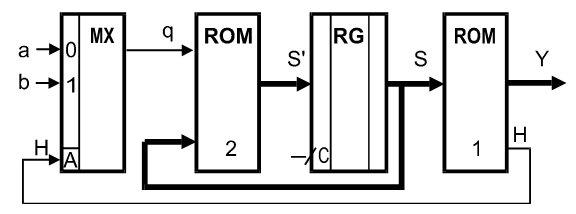
\includegraphics[width=0.7\linewidth]{line_rom}
		\caption{УА с адресным ПЗУ; последовательный вариант}
		\label{img:scheme1}
	\end{center}	
\end{figure}

В конкретной реализации роль мультиплексора выполняет логический элемент ИЛИ, на входы которого подаются сигналы $CT0$~---~признак нуля в счетчике и осведомительный сигнал (признак) $H$~---~указывающий на присутствие логического ветвления в текущем месте алгоритма.

\subsection{Алгоритм работы автомата}
Опишем алгоритм работы автомата с помощью блок схемы. Используем сумматор для сложения текущего значение СЧП и множимого, счетчик для подсчета обработанных разрядов и регистры для хранения и использования разрядов рассматриваемых чисел. Обозначим микрокоманды от $m_0$ до $m_4$. См. рисунок~\ref{img:algorithm1}.\vspace{2ex}

\begin{figure}[h!]
	\centering
	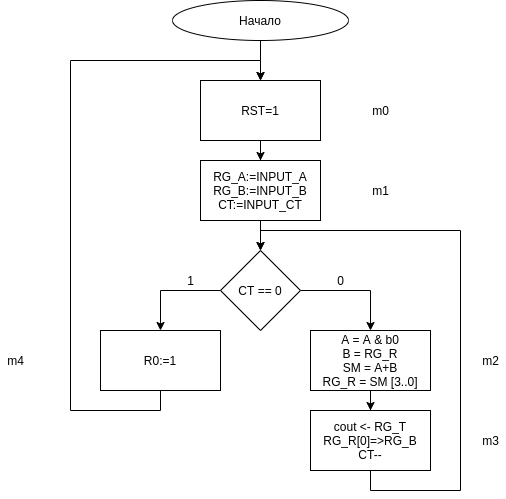
\includegraphics[width=0.7\linewidth]{algorithm}
	\caption {Алгоритм умножения двух 4-разрядных чисел}
	\label{img:algorithm1}
\end{figure}

В алгоритме присутствует условие, это означает, что при реализации операционного автомата текущие значение счетчика необходимо проверять при переходе $m_0 \to m_1$ и $m_3 \to m_1$.

После построения алгоритма работы автомата следует перейти к реализации операционной части.

\subsection {Реализация Операционного автомата}
Построим операционный автомат, выполняющий умножение двух 4-разрядных чисел посредством использования четырех регистров, в том числе двух сдвиговых. Приведем названия и назначения каждого из регистров. См. таблицу \ref{tab:regs1}.
\begin{table}[h!]
	\centering
	\begin{tabular}{|p{0.27\linewidth}|p{0.6\linewidth}|}
		\hline
		\textbf{Идентификатор} & \textbf{Назначение} \\ \hline
		$RG\_A$ & Хранит разряды множимого \\ \hline
		$RG\_B$ & Сдивговый регистр. Хранит разряды множителя \\ \hline
		$RG\_R$ & Cдвиговый регистр. Хранит разряды СЧП, служит для хранения старших разрядов результата \\ \hline
		$RG\_D$ & Сдвиговый регистр. Хранит младшие разряды результата \\ \hline
	\end{tabular}
	\caption{Регистры операционного автомата}
	\label{tab:regs1}
\end{table}

Укажем необходимые признаки, которые впоследствии будут вырабатываться управляющим автоматом. См. таблицу \ref{tab:signals1}.
\begin{table}[h!]
	\centering
	\begin{tabular}{|p{0.27\linewidth}|p{0.6\linewidth}|}
		\hline
		\textbf{Признак} & \textbf{Назначение} \\ \hline
		$Н$ & Указывает на условность--безусловность перехода \\ \hline
		$EMIT\_R_0$ & Сигнализирует об окончании операции умножения \\ \hline
		$LOAD\_R$ & Загрузка в регистр $RG\_R$ \\ \hline
		$RST$ & Асинхронный сброс всех элементов \\ \hline
		$COUNT\_CT$ & Загрузка счетчика. Декремент, если $DECR\_CT==1$ \\ \hline
		$DECR\_CT$ & Декремент счетчика \\ \hline
		$LOAD\_AB$ & Загрузка в регистры $RG\_A \text{ и } RG\_B$ \\ \hline
		$SHIFT\_RB$ & Сдвиг в регистрах $RG\_R \text{ и } RG\_B$ \\ \hline
	\end{tabular}
	\caption{Осведомительные сигналы (признаки)}
	\label{tab:signals1}
\end{table}
Соединим все элементы в соответствии с алгоритмом задачи. См. рисунок \ref{img:oa1}.

\begin{figure}[h!]
	\centering
	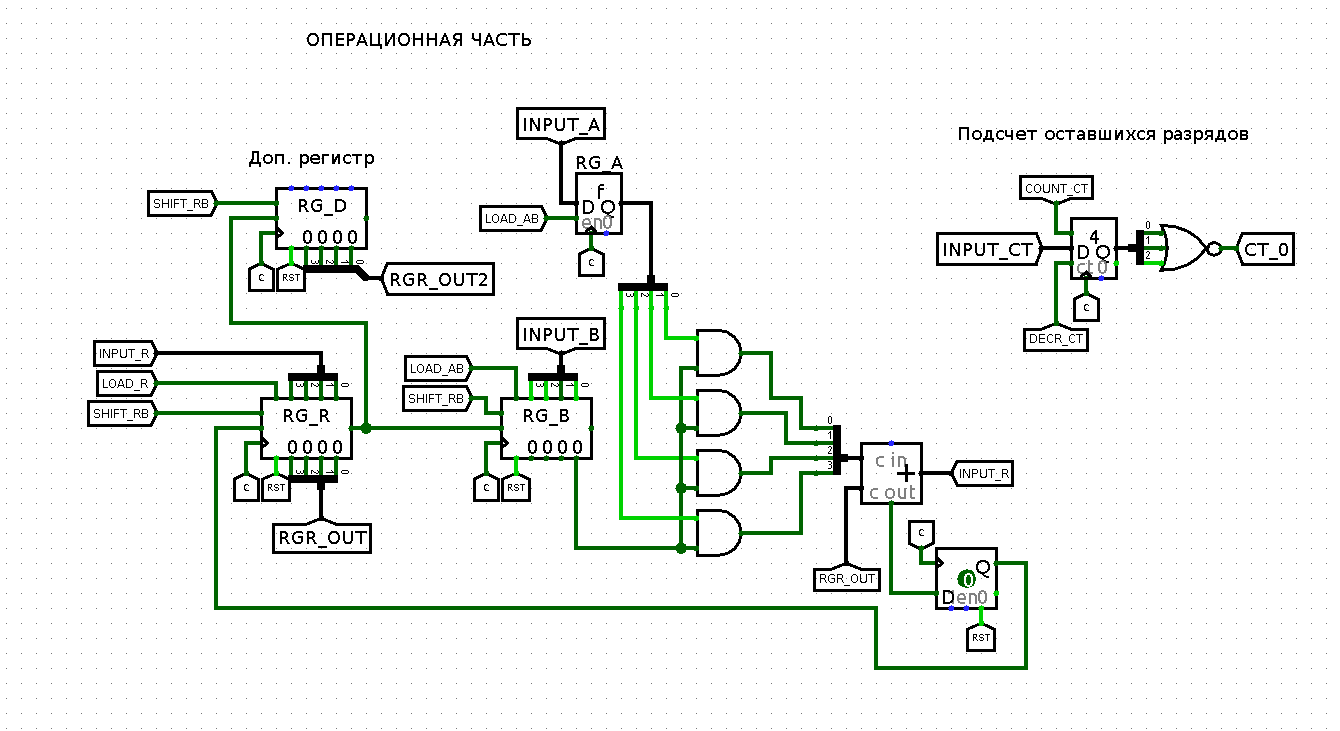
\includegraphics[width=\linewidth]{OA}
	\caption {Схема операционного автомата}
	\label{img:oa1}
\end{figure}
\newpage
\subsection {Реализация управляющего автомата}
Приступим к построению управляющего автомата, определяющего последовательность выполнения микрокоманд для умножения двух 4-разрядных чисел. 

Определим разрядность адресного ПЗУ и ПЗУ микрокоманд. Адрес должен иметь 4 разряда, где ведущим разряд~--- текущее значение параметра \textit{CT0}. Микрокоманда представлена в виде 8 бит~--- 8 признаков, расположенных в следующем порядке: H, EMIT\_R0, LOAD\_R, RST, CONT\_CT, DECR\_CT, LOAD\_AB, SHIFT\_RB. Адрес текущей команды будет храниться в 4-разрядном регистре.


Заполним память в соответствии в алгоритмом, подключим ПЗУ и регистр последовательным способом. См рисунок \ref{img:ma1}.
\begin{figure}[h!]
	\centering
	\includegraphics[width=0.7\linewidth]{MA}
	\caption {Схема операционного автомата}
	\label{img:ma1}
\end{figure}

\subsection{Тестирование работы автомата}
После реализации операционного и управляющего автомата следует приступить к объединению данных устройств, тестированию их совместной работы. Подключим признаки к входам соответствующих логических элементов и цифровых устройств с помощью туннелей. Добавим блок ввода исходных данных, используя контакты, блок вывода~---регистр результата и индикатор завершения операции умножения.

Проведем проверку корректности выходных результатов построенного цифрового устройства. Перемножим два наибольших 4-разрядных двоичных числа $1111_2 \ast 1111_2$ ожидая получить двоичное число $11100001_2$. Укажем входные данные, будем подавать тактовые сигналы до тех пор, пока индикатор не сообщит нам о завершении операции, сравним практические результаты с ожидаемыми. См рисунок~\ref{img:test1}. Умножение выполнено корректно. Ожидаемые и полученные результаты совпадают.
\begin{figure}[h!]
	\centering
	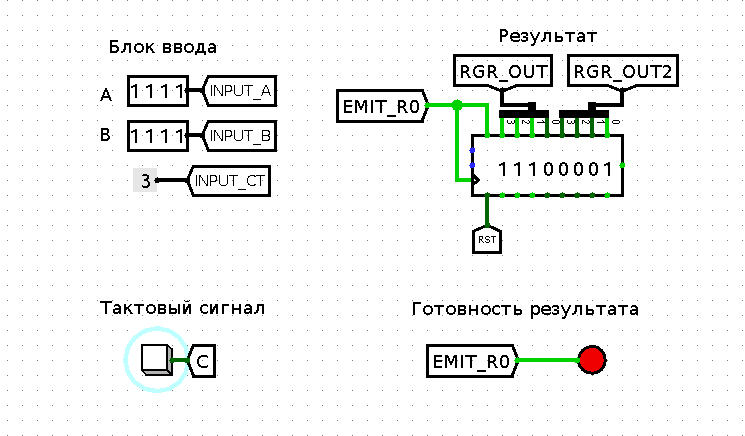
\includegraphics[width=0.7\linewidth]{test}
	\caption {Схема операционного автомата}
	\label{img:test1}
\end{figure}

\subsection {Вывод}
В ходе данной практической работы было рассмотрено строение и работа управляющего автомата с адресным ПЗУ. Использовав полученные знания на практике, на основе данного управляющего автомата построено вычислительное устройство (операционный и управляющий автомат), реализующее операцию умножения двух 4-разрядных чисел без знака. Работа данного устройства испытана, проверена корректность полученных результатов. 
\newpage
\section {Практическая работа №2.\\Умножитель 4-разрядных чисел в дополнительном коде }
\subsection{Общее строение автомата}
В ходе данной практической работы был реализован автомат, выполняющий умножение 4-разрядных чисел в дополнительном коде. Управляющий автомат был построен по схеме с двумя адресами в памяти в последовательном варианте. Рассмотрим строение управляющего автомата. См рисунок~\ref{img:scheme2}.

\begin{figure}[h!]
	\begin{center}
		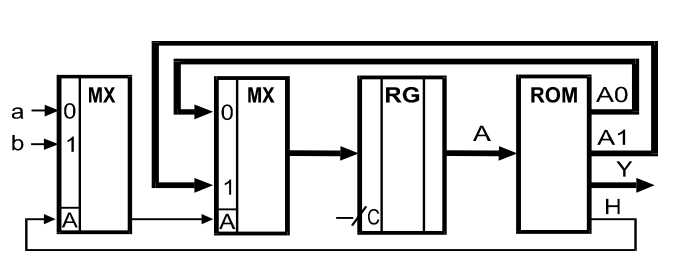
\includegraphics[width=0.7\linewidth]{two_adress_rom}
		\caption{УА с двумя адресами в памяти; последовательный вариант}
		\label{img:scheme2}
	\end{center}	
\end{figure}

В конкретной реализации на адресный вход мультиплексора подается сигнал \textit{CT0}~---~признак нуля в счетчике. Основываясь на значении данного сигнала выбирается один из двух альтернативных адресов последующих состояний автомата.

\subsection{Алгоритм работы автомата}
Опишем алгоритм работы автомата с помощью блок схемы. Используем сумматор для сложения текущего значение СЧП и множимого, счетчик для подсчета обработанных разрядов и регистры для хранения и использования разрядов рассматриваемых чисел. Обозначим микрокоманды от $m_0$ до $m_4$. См. рисунок~\ref{img:algorithm2}.\vspace{2ex}

\begin{figure}[h!]
	\centering
	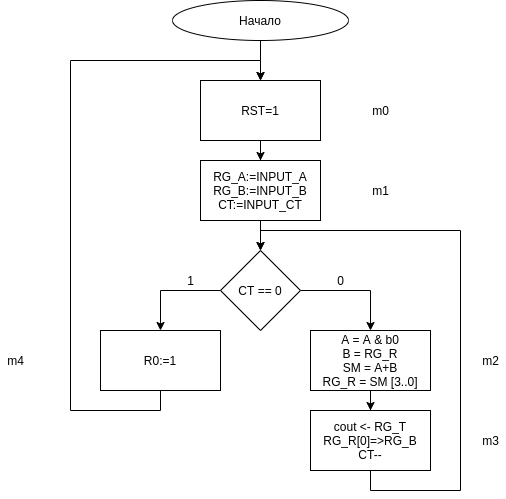
\includegraphics[width=0.7\linewidth]{algorithm}
	\caption {Алгоритм умножения двух 4-разрядных чисел}
	\label{img:algorithm2}
\end{figure}

В алгоритме присутствует условие, это означает, что при реализации операционного автомата текущие значение счетчика необходимо проверять при переходе $m_0 \to m_1$ и $m_3 \to m_1$.

После построения алгоритма работы автомата следует перейти к реализации операционной части.

\subsection {Реализация Операционного автомата}
Построим операционный автомат, выполняющий умножение двух 4-разрядных чисел посредством использования четырех регистров, в том числе двух сдвиговых. Приведем названия и назначения каждого из регистров. См. таблицу \ref{tab:regs2}.
\begin{table}[h!]
	\centering
	\begin{tabular}{|p{0.27\linewidth}|p{0.6\linewidth}|}
		\hline
		\textbf{Идентификатор} & \textbf{Назначение} \\ \hline
		$RG\_A$ & Хранит разряды множимого \\ \hline
		$RG\_B$ & Сдивговый регистр. Хранит разряды множителя \\ \hline
		$RG\_R$ & Cдвиговый регистр. Хранит разряды СЧП, служит для хранения старших разрядов результата \\ \hline
	\end{tabular}
	\caption{Регистры операционного автомата}
	\label{tab:regs2}
\end{table}

Укажем необходимые признаки, которые впоследствии будут вырабатываться управляющим автоматом. См. таблицу \ref{tab:signals2}.
\begin{table}[hbtp]
	\centering
	\begin{tabular}{|p{0.27\linewidth}|p{0.6\linewidth}|}
		\hline
		\textbf{Признак} & \textbf{Назначение} \\ \hline
		$EMIT\_R_0$ & Сигнализирует об окончании операции умножения \\ \hline
		$LOAD\_R$ & Загрузка в регистр $RG\_R$ \\ \hline
		$RST$ & Асинхронный сброс всех элементов \\ \hline
		$COUNT\_CT$ & Загрузка счетчика. Декремент, если $DECR\_CT==1$ \\ \hline
		$DECR\_CT$ & Декремент счетчика \\ \hline
		$LOAD\_AB$ & Загрузка в регистры $RG\_A \text{ и } RG\_B$ \\ \hline
		$SHIFT\_RB$ & Сдвиг в регистрах $RG\_R \text{ и } RG\_B$ \\ \hline
	\end{tabular}
	\caption{Осведомительные сигналы (признаки)}
	\label{tab:signals2}
\end{table}

При умножении по данному алгоритму следует обратить внимание на необходимость использования модифицированного дополнительного кода для множимого, поскольку при получении частичных произведений возможно временное переполнение разрядной сетки. Использование модифицированного дополнительного кода позволяет его зафиксировать без потери знака. Это переполнение устраняется последующим сдвигом частичного произведения вправо. 

\begin{figure}[h!]
	\centering
	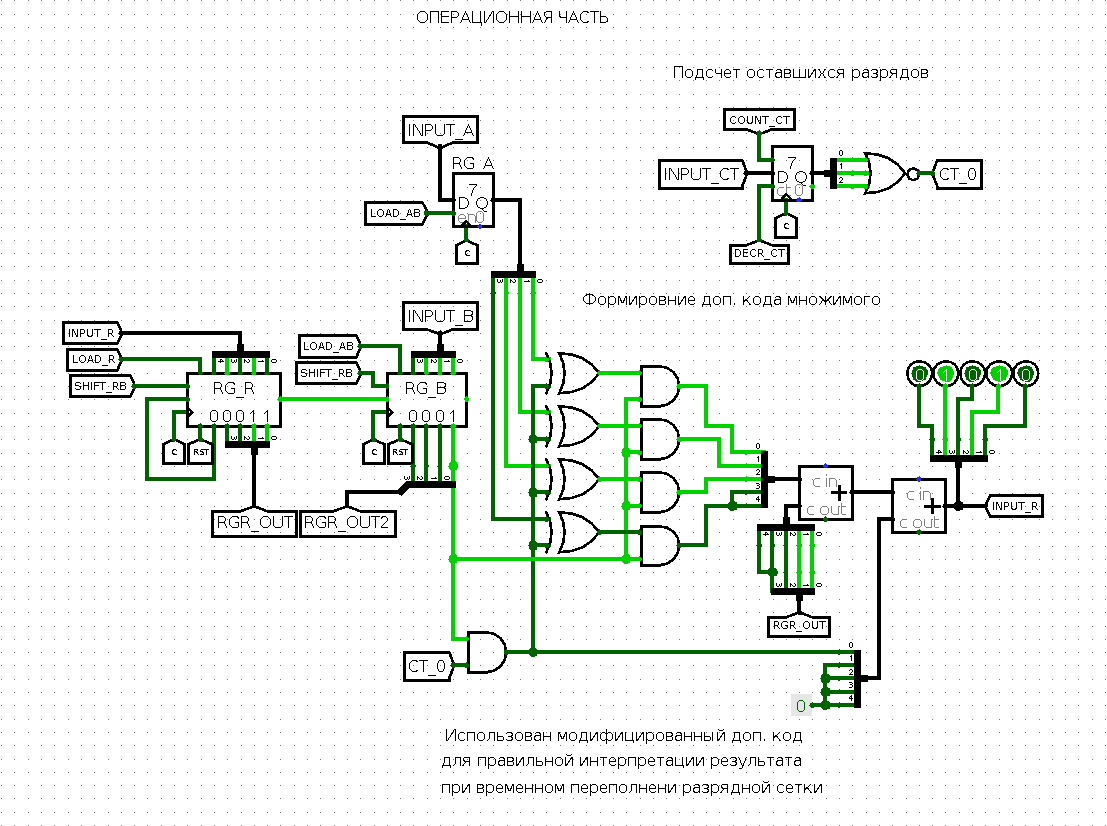
\includegraphics[width=0.6\linewidth]{OA_two_adress}
	\caption {Схема операционного автомата}
	\label{img:oa2}
\end{figure}

Соединим все элементы в соответствии с алгоритмом задачи. См. рисунок \ref{img:oa2}.

\subsection {Реализация управляющего автомата}
Приступим к построению управляющего автомата, определяющего последовательность выполнения микрокоманд для умножения двух 4-разрядных чисел в дополнительном коде.

Определим разрядность ПЗУ, в котором будут содержаться альтернативные адреса переходов. Микроинструкция представлена в виде 13 разрядов, где 6 разрядов занимают два альтернативных адреса переходов, а оставшиеся 7~--- признаки, расположенные в следующем порядке: RST, SHIFT\_RB, LOAD\_AB, LOAD\_R, DECR\_CT, CONT\_CT, EMIT\_R0. Адрес текущей команды будет храниться в 3-разрядном регистре.

Альтернативные адреса будут подаваться на вход мультиплексора, управляемого сигналом \textit{CT0}, затем, выбранный адрес будет загружен в регистр текущего состояния, выход которого подключен к постоянному запоминающему устройству.


Заполним память в соответствии в алгоритмом, подключим ПЗУ и регистр последовательным способом. См рисунок \ref{img:ma2}.
\begin{figure}[htbp]
	\centering
	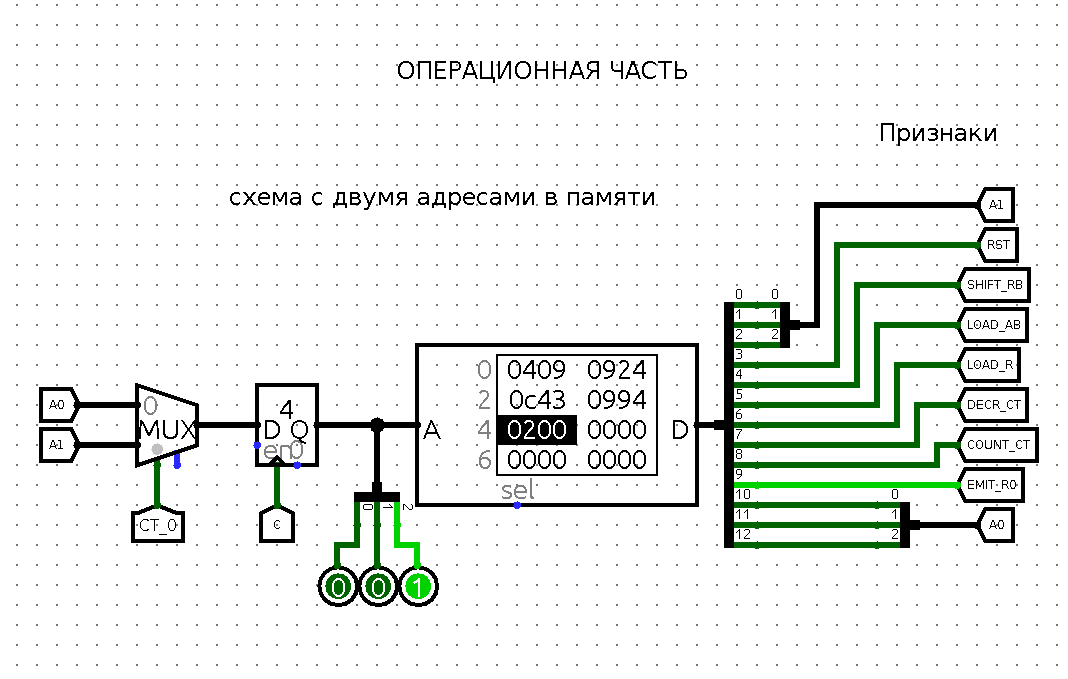
\includegraphics[width=0.8\linewidth]{MA_two_adress}
	\caption {Схема операционного автомата}
	\label{img:ma2}
\end{figure}

\subsection{Тестирование работы автомата}
После реализации операционного и управляющего автомата следует приступить к объединению данных устройств, тестированию их совместной работы. Подключим признаки к входам соответствующих логических элементов и цифровых устройств с помощью туннелей. Добавим блок ввода исходных данных, используя контакты, блок вывода~---регистр результата и индикатор завершения операции умножения.

Проведем проверку корректности выходных результатов построенного цифрового устройства. Перемножим два  4-разрядных двоичных числа $1111_{доп_2} \ast 1111_{доп_2}$, которые в данном случае интерпретируются как дополнительный код отрицательного десятичного числа $-1_{10}$ ожидая получить результат $-1_{10} = 00000001_{доп_2}$. Укажем входные данные, будем подавать тактовые сигналы до тех пор, пока индикатор не сообщит нам о завершении операции, сравним практические результаты с ожидаемыми. См рисунок~\ref{img:test2.1}. Умножение выполнено корректно. Ожидаемые и полученные результаты совпадают.
\begin{figure}[h!]
	\centering
	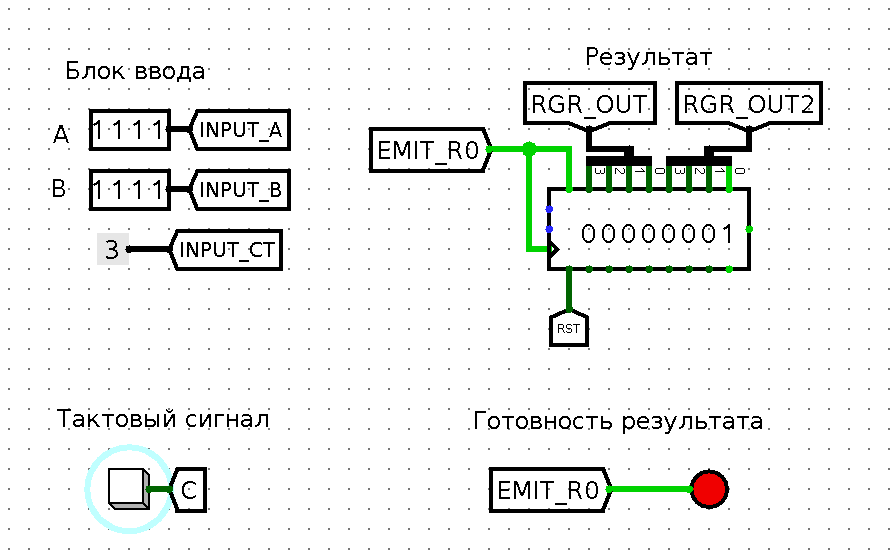
\includegraphics[width=0.7\linewidth]{test_two_adress}
	\caption {Схема операционного автомата}
	\label{img:test2.1}
\end{figure}

Теперь перемножим положительное число $7_{10}=0111_{доп_2}$ и отрицательное число $-2_{10}=1110_{доп_2}$, ожидая получить результат $-14_{10}=11110010_{доп_2}$. Введем исходные данные и сравним результаты вычислений. См. рисунок \ref{img:test2.2}. Как видно на рисунке, вычисления привели к верному ответу. С помощью данного автомата можно перемножать числа в диапазоне $(-7;7)$.
\begin{figure}[h!]
	\centering
	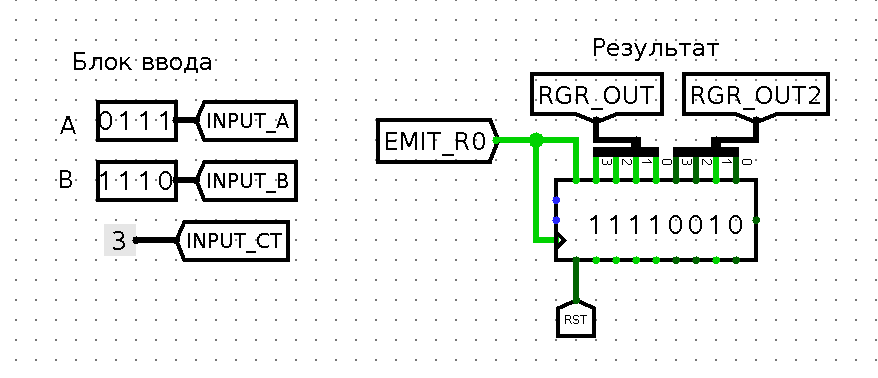
\includegraphics[width=0.7\linewidth]{test_two_adress1}
	\caption {Схема операционного автомата}
	\label{img:test2.2}
\end{figure}

\subsection {Вывод}
В ходе данной практической работы было рассмотрено строение и работа последовательного варианта управляющего автомата c двумя адресами в памяти. Использовав полученные знания на практике, на основе данного управляющего автомата построено вычислительное устройство (операционный и управляющий автомат), реализующее операцию умножения двух 4-разрядных чисел в дополнительном коде. Работа данного устройства испытана, проверена корректность полученных результатов.
\newpage
\section {Практическая работа №3.\\Делитель 4-разрядных чисел без знака }

\subsection{Общее строение автомата}
В ходе данной практической работы был реализован автомат, выполняющий деление 4-разрядных чисел без знака (алгоритм без восстановления остатка). Управляющий автомат был построен по схеме с одним адресом в памяти в последовательном варианте. Рассмотрим строение управляющего автомата. См рисунок~\ref{img:scheme3}.

\begin{figure}[h!]
	\begin{center}
		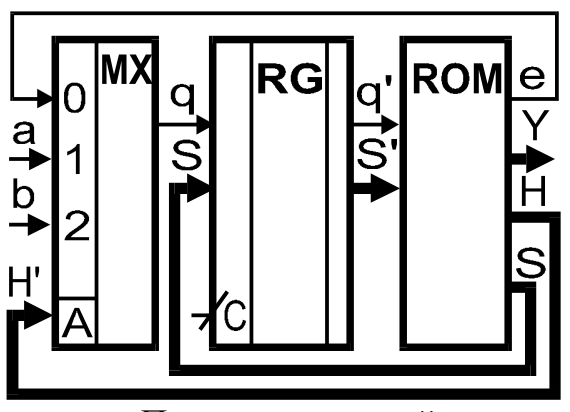
\includegraphics[width=0.5\linewidth]{one_adress_rom}
		\caption{УА с одним адресом в памяти; последовательный вариант}
		\label{img:scheme3}
	\end{center}	
\end{figure}

В конкретной реализации на информационные входы мультиплексора подаются сигналы \textit{e} -- сигнал с ПЗУ, \textit{B\_IS\_NULL} -- признак нулевого делителя, \textit{CT\_IS\_NULL} -- признак окончания счета, \textit{b\_high} -- значение старшего бита частичного остатка на текущей итерации, а на адресный вход подается двухбитовый сигнал \textit{H}.
\subsection{Алгоритм работы автомата}
Опишем алгоритм работы автомата с помощью блок схемы. Используем сумматор для нахождения текущего значение частичного остатка (ЧО), счетчик для подсчета обработанных разрядов и регистры для хранения и использования разрядов делителя и делимого. Обозначим микрокоманды от $m_0$ до $m_4$. См. рисунок~\ref{img:algorithm3} в \hyperref[tam]{Приложении~А}.

После построения алгоритма работы автомата следует перейти к реализации операционной части.

\subsection {Реализация Операционного автомата}
Построим операционный автомат, выполняющий деление двух 4-разрядных чисел посредством использования четырех регистров, в том числе трех сдвиговых. Приведем названия и назначения каждого из регистров. См. таблицу \ref{tab:regs3}.
\begin{table}[h!]
	\centering
	\begin{tabular}{|m{0.27\linewidth}|m{0.6\linewidth}|}
		\hline
		\textbf{Идентификатор} & \textbf{Назначение} \\ \hline
		$RG\_A$ & Сдвиговый регистр. Хранит разряды делимого \\ \hline
		$RG\_B$ & Хранит разряды делителя \\ \hline
		$RG\_REM$ & Сдвиговый регистр. Хранит разряды частичного остатка \\ \hline
		$RG\_RES$ & Сдвиговый регистр. Хранит разряды результата \\ \hline
	\end{tabular}
	\caption{Регистры операционного автомата}
	\label{tab:regs3}
\end{table}

Укажем необходимые признаки, которые впоследствии будут вырабатываться управляющим автоматом. См. таблицу \ref{tab:signals3}.
\begin{table}[h!]
	\centering
	\begin{tabular}{|m{0.27\linewidth}|m{0.6\linewidth}|}
		\hline
		\textbf{Признак} & \textbf{Назначение} \\ \hline
		$S$ & Хранит адрес следующей операции \\ \hline
		$Н$ & Адресный вход мультиплексора \\ \hline
		$R0$ & Сигнализирует об окончании операции деления \\ \hline
		$ERROR$ & Сигнализирует об ошибке ввода -- делитель равен нулю \\ \hline
		$L\_RG_A$ & Загрузка в регистр $RG\_A$ \\ \hline
		$L\_RG_B$ & Загрузка в регистр $RG\_B$ \\ \hline
		$L\_RG_REM$ & Загрузка в регистр $RG\_REM$ \\ \hline
		$CLR$ & Асинхронный сброс всех элементов \\ \hline
		$COUNT\_CT$ & Счет. Декремент счетчика, если $L\_CT==1$ \\ \hline
		$L\_CT$ & Загрузка счетчика \\ \hline
		$SHIFT$ & Левый сдвиг в регистрах $RG\_A \text{ и } RG\_RES$ \\ \hline
	\end{tabular}
	\caption{Осведомительные сигналы (признаки)}
	\label{tab:signals3}
\end{table}
С целью реализации левого сдвига в сдвиговых регистрах разряды делимого и текущего значения частичного остатка загружаются в регистры в обратном порядке. Это позволяет отказаться от универсального сдвигового регистра, так как реализации данного алгоритма необходим только левый сдвиг, и как следствие, упрощает схему. 

Для исключения возникновения ошибки при левом сдвиге разрядов частичного остатка в случае, когда два его старших разряда различны, использованы 6-разрядные регистры. См. сноску \ref{sign3}.

Соединим все элементы в соответствии с алгоритмом задачи. См. рисунок \ref{img:oa3} в приложении \hyperref[tam]{Приложении А}.
\begin{equation}
\begin{aligned}
\label{sign3}
-|B| &\neq 10X...X \\
-|B| &= 110X...X
\end{aligned}
\end{equation}
\subsection {Реализация управляющего автомата}
Приступим к построению управляющего автомата, определяющего последовательность выполнения микрокоманд для деления двух 4-разрядных чисел без знака.

Определим разрядность ПЗУ, участвующего в построении УА по схеме с одним адресом в памяти. Адрес должен иметь 4 разряда, где 3 старших разряда~--- текущее значение параметра \textit{S}, а младший разряд~--- значение $q$, генерируемое мультиплексором. Микрокоманда представлена в виде 15 бит~--- 12 признаков, расположенных в следующем порядке:\hspace{0ex}$S, H, R0, ERROR, CLR,$ $L\_CT,$ $COUNT\_CT,$ $SHIFT,$ $L\_RG\_REM, L\_RG_B, L\_RG_A, e$. Адрес текущей команды будет храниться в 4-разрядном регистре.


Заполним память в соответствии в алгоритмом, подключим ПЗУ и регистр последовательным способом. См рисунок \ref{img:ma3}.
\begin{figure}[h!]
	\centering
	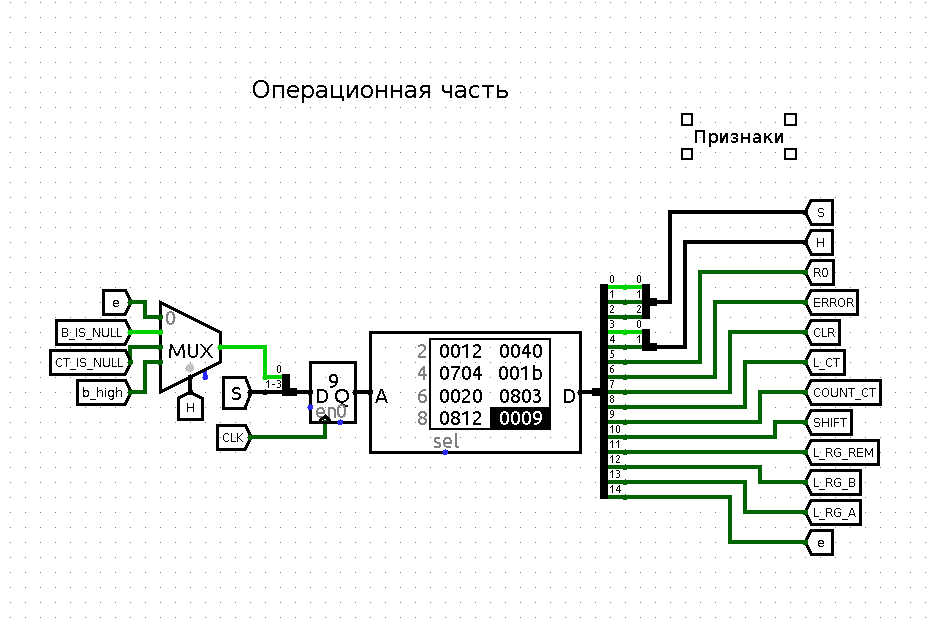
\includegraphics[width=0.7\linewidth]{MA3}
	\caption {Схема операционного автомата}
	\label{img:ma3}
\end{figure}

\subsection{Тестирование работы автомата}
После реализации операционного и управляющего автомата следует приступить к объединению данных устройств, тестированию их совместной работы. Подключим признаки к входам соответствующих логических элементов и цифровых устройств с помощью туннелей. Добавим блок ввода исходных данных, используя контакты, блок вывода~---регистр результата операции деления и регистр остатка, индикатор завершения операции деления.

Проведем проверку корректности выходных результатов построенного цифрового устройства. Разделим два наибольших 4-разрядных двоичных числа $1111_2 \div 1111_2$ ожидая получить частное $1_2$ и остаток $0_2$ . Укажем входные данные, будем подавать тактовые сигналы до тех пор, пока индикатор не сообщит нам о завершении операции, сравним практические результаты с ожидаемыми. См рисунок~\ref{img:test3.1}. Умножение выполнено корректно. Ожидаемые и полученные результаты совпадают.
\begin{figure}[h!]
	\centering
	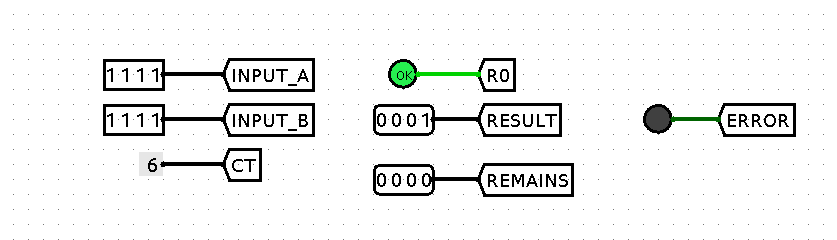
\includegraphics[width=0.6\linewidth]{test3.1}
	\caption {Проверка работы автомата}
	\label{img:test3.1}
\end{figure}

Протестируем работу автомата на входных данных, которые гипотетически могут привести к ошибке --- поделим число $101_2$ на число $1111_2$. Ошибка состоит в том, что в случае использования регистров недостаточной разрядности, левый сдвиг при вычислении очередного остатка произойдет некорректно, что приведет к неверному результату. Введем данные, пронаблюдаем за работой автомата. См рисунок \ref{img:test3.2}. Операция выполнена верно. Использование регистров большей разрядности исключило возможность ошибки.
\begin{figure}[h!]
	\centering
	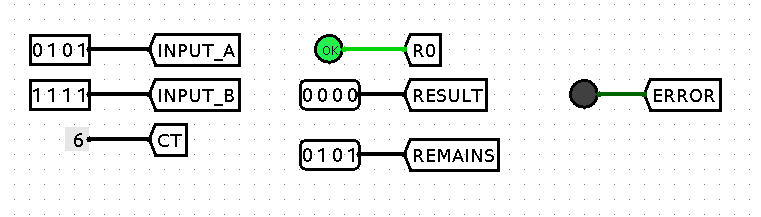
\includegraphics[width=0.6\linewidth]{test3.2}
	\caption {Вторая проверка работы автомата}
	\label{img:test3.2}
\end{figure}
\subsection {Вывод}
В ходе данной практической работы было рассмотрено строение и работа управляющего автомата, построенного по схеме с одним адресом в памяти. Использовав полученные знания на практике, на основе данного управляющего автомата построено вычислительное устройство (операционный и управляющий автомат), реализующее операцию деления двух 4-разрядных чисел без знака.

Работа данного устройства испытана, проверена корректность полученных результатов при работе со всеми категориями входных данных. 
\newpage
\section {Практическая работа №4.\\Делитель 4-разрядных чисел в дополнительном коде}
\subsection{Общее строение автомата}
В ходе данной практической работы был реализован автомат, выполняющий деление 4-разрядных чисел в дополнительном коде (алгоритм без восстановления остатка). Управляющий автомат был построен по схеме с сокращенным тактом. Рассмотрим строение управляющего автомата. См рисунок~\ref{img:scheme4}.

\begin{figure}[h!]
	\begin{center}
		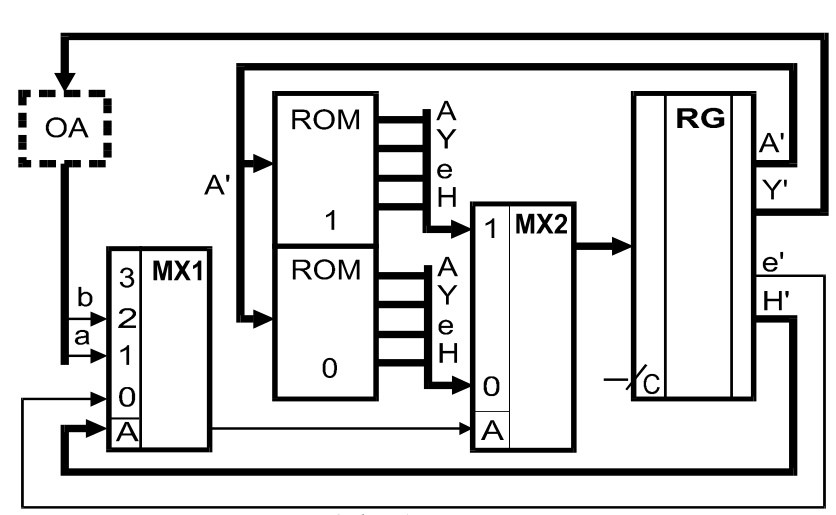
\includegraphics[width=0.5\linewidth]{short_cycle_rom}
		\caption{УА с сокращенным тактом}
		\label{img:scheme4}
	\end{center}	
\end{figure}

В конкретной реализации на информационные входы мультиплексора подаются сигналы \textit{e} -- сигнал с ПЗУ, \textit{B\_IS\_NULL} -- признак нулевого делителя, \textit{CT\_IS\_NULL} -- признак окончания счета, \textit{b\_high} -- значение старшего бита частичного остатка на текущей итерации, а на адресный вход подается двухбитовый сигнал \textit{H}.
\subsection{Алгоритм работы автомата}
Опишем алгоритм работы автомата с помощью блок схемы. Используем сумматор для нахождения текущего значение частичного остатка (ЧО), счетчик для подсчета обработанных разрядов и регистры для хранения и использования разрядов делителя и делимого. Обозначим микрокоманды от $m_0$ до $m_4$. См. рисунок~\ref{img:algorithm4} в \hyperref[tam]{Приложении~А}.

После построения алгоритма работы автомата следует перейти к реализации операционной части.

\subsection {Реализация Операционного автомата}
Построим операционный автомат, выполняющий деление двух 4-разрядных чисел в дополнительном коде посредством использования четырех регистров, в том числе трех сдвиговых. Приведем названия и назначения каждого из регистров. См. таблицу \ref{tab:regs4}.
\begin{table}[h!]
	\centering
	\begin{tabular}{|m{0.27\linewidth}|m{0.6\linewidth}|}
		\hline
		\textbf{Идентификатор} & \textbf{Назначение} \\ \hline
		$RG\_A$ & Сдвиговый регистр. Хранит разряды делимого \\ \hline
		$RG\_B$ & Хранит разряды делителя \\ \hline
		$RG\_REM$ & Сдвиговый регистр. Хранит разряды частичного остатка \\ \hline
		$RG\_RES$ & Сдвиговый регистр. Хранит разряды результата \\ \hline
	\end{tabular}
	\caption{Регистры операционного автомата}
	\label{tab:regs4}
\end{table}

Укажем необходимые признаки, которые впоследствии будут вырабатываться управляющим автоматом. См. таблицу \ref{tab:signals4}.
\begin{table}[h!]
	\centering
	\begin{tabular}{|m{0.27\linewidth}|m{0.6\linewidth}|}
		\hline
		\textbf{Признак} & \textbf{Назначение} \\ \hline
		$S$ & Хранит адрес следующей операции \\ \hline
		$Н$ & Адресный вход мультиплексора \\ \hline
		$R0$ & Сигнализирует об окончании операции деления \\ \hline
		$ERROR$ & Сигнализирует об ошибке ввода -- делитель равен нулю \\ \hline
		$L\_RG_A$ & Загрузка в регистр $RG\_A$ \\ \hline
		$L\_RG_B$ & Загрузка в регистр $RG\_B$ \\ \hline
		$L\_RG_REM$ & Загрузка в регистр $RG\_REM$ \\ \hline
		$CLR$ & Асинхронный сброс всех элементов \\ \hline
		$COUNT\_CT$ & Счет. Декремент счетчика, если $L\_CT==1$ \\ \hline
		$L\_CT$ & Загрузка счетчика \\ \hline
		$SHIFT$ & Левый сдвиг в регистрах $RG\_A \text{ и } RG\_RES$ \\ \hline
	\end{tabular}
	\caption{Осведомительные сигналы (признаки)}
	\label{tab:signals4}
\end{table}
С целью реализации левого сдвига в сдвиговых регистрах разряды делимого и текущего значения частичного остатка загружаются в регистры в обратном порядке. Это позволяет отказаться от универсального сдвигового регистра, так как реализации данного алгоритма необходим только левый сдвиг, и как следствие, упрощает схему. 

Для исключения возникновения ошибки при левом сдвиге разрядов частичного остатка в случае, когда два его старших разряда различны, использованы 6-разрядные регистры. См. сноску \ref{sign4}.

\begin{equation}
\begin{aligned}
\label{sign4}
-|B| &\neq 10X...X \\
-|B| &= 110X...X
\end{aligned}
\end{equation}

Стоит отметить, что для формирования правильного выходного результата необходимо выполнить коррекцию значений частного и остатка в зависимости от знаков операндов. Для каждой комбинации знаков делимого и делителя реализована отдельная операция коррекции. См таблицу \ref{tab:correction4}.

\begin{table}
	\begin{tabular}{|m{0.2\linewidth}|m{0.67\linewidth}|}
		\hline
		\textbf{Комбинация} &\textbf{Коррекция}\\
		\hline
		$A\ge0, B>0 $ & Коррекция не требуется \\ 
		\hline
		$A\ge0, B<0$ & Перевести частное в доп. код\\
		\hline
		$A\le0, B>0$ & Результат верен, если остаток $=0$. Иначе прибавить к отрицательному частному единицу, перевести остаток в доп. код\\
		\hline
		$A\le 0, B\le 0$ & Изменить знак делимого, перевести остаток в доп. код\\
		\hline
	\end{tabular}
	\caption{Коррекция результата}
	\label{tab:correction4}
\end{table}

Соединим все элементы в соответствии с алгоритмом задачи. См. рисунки \ref{img:oa4.1} и \ref{img:oa4.2} в приложении \hyperref[tam]{Приложении А}.

\subsection {Реализация управляющего автомата}
Приступим к построению управляющего автомата, определяющего последовательность выполнения микрокоманд для деления двух 4-разрядных чисел в дополнительном коде.

Определим разрядность двух ПЗУ, участвующих в построении УА по схеме с сокращенным тактом. Адрес должен иметь 3 разряда~--- текущее значение параметра \textit{S}. Микрокоманда представлена в виде 15 бит~--- 12 признаков, расположенных в следующем порядке:\hspace{-1ex}$S, H, R0, ERROR,$ $CLR,$ $L\_CT,$ $COUNT\_CT,$ $SHIFT,$ $L\_RG\_REM,$ $L\_RG_B, L\_RG_A, e$. Текущая команда хранится в 15~ти разрядом регистре. В первом ПЗУ, имеющем метку <<0>> будут хранится микрокоманды, вторая часть адреса которых содержит нулевой бит. Автомат переходит в эти состояния, когда условия, заключенные в операторе выбора, отображенном на диаграмме, не выполняются. Второй ПЗУ с меткой <<1>> хранит микрокоманды, в которые автомат переходит при выполнении условий, заключенных в операторе выбора. Данные микрокоманды имеют единичный бит во второй части адреса.

Микрокоманды, расположенные в ПЗУ по текущему адресу попадают на вход мультиплексора, адресным входом которого является значение признака, рассматриваемого в текущем состоянии.

Заполним память в соответствии в алгоритмом, подключим ПЗУ, мультиплексоры и регистр последовательным способом. См рисунок \ref{img:ma4} в \hyperref[tam]{Приложении А}.


\subsection{Тестирование работы автомата}
После реализации операционного и управляющего автомата следует приступить к объединению данных устройств и тестированию их совместной работы. Подключим признаки к входам соответствующих логических элементов и цифровых устройств с помощью туннелей. Добавим блок ввода исходных данных, используя контакты, блок вывода~---регистр результата операции деления и регистр остатка, индикатор завершения операции деления.

Проведем проверку корректности выходных результатов построенного цифрового устройства. Разделим два наибольших 4-разрядных двоичных числа $1111_2 \div 1111_2$ ожидая получить частное $1_2$ и остаток $0_2$ . Укажем входные данные, будем подавать тактовые сигналы до тех пор, пока индикатор не сообщит нам о завершении операции, сравним практические результаты с ожидаемыми. См рисунок~\ref{img:test4.1}. Умножение выполнено корректно. Ожидаемые и полученные результаты совпадают.
\begin{figure}[h!]
	\centering
	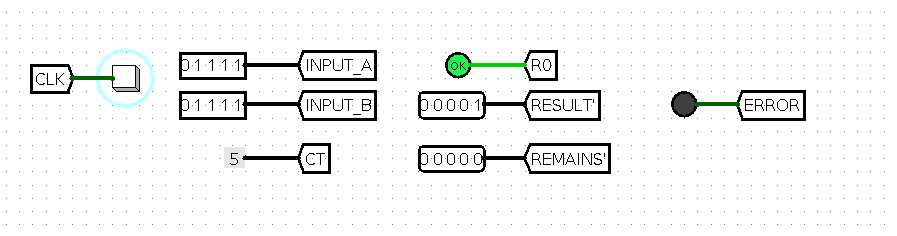
\includegraphics[width=0.6\linewidth]{test4.1}
	\caption {Проверка работы автомата}
	\label{img:test4.1}
\end{figure}

Протестируем работу автомата на входных данных, которые гипотетически могут привести к ошибке --- поделим число $101_2$ на число $1111_2$. Ошибка состоит в том, что в случае использования регистров недостаточной разрядности, левый сдвиг при вычислении очередного остатка произойдет некорректно, что приведет к неверному результату. Введем данные, пронаблюдаем за работой автомата. См рисунок \ref{img:test4.2}. Операция выполнена верно. Использование регистров большей разрядности исключило возможность ошибки.
\begin{figure}[h!]
	\centering
	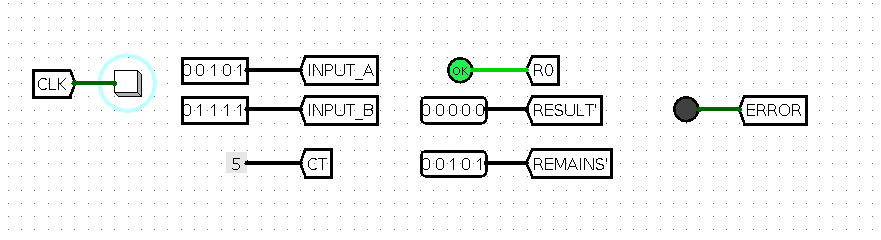
\includegraphics[width=0.6\linewidth]{test4.2}
	\caption {Вторая проверка работы автомата}
	\label{img:test4.2}
\end{figure}

Проведем тестирование работы автомата на отрицательных числах. Рассмотрим три варианта, при которых:
\begin{enumerate}
	\item Делимое неотрицательно, делитель отрицателен;
	\item Делимое отрицательно, делитель положителен;
	\item Делимое отрицательно, делитель отрицателен.
\end{enumerate}
Рассмотрим конкретные примеры.
\vspace{2ex}\\
\begin{tabularx}{\linewidth}{|c|c|X|X|X|}%{|c|m{0.2\linewidth}|m{0.33\linewidth}|m{0.33\linewidth}|}
	\hline
	\textbf{№} &\multicolumn{2}{c|}{\textbf{Комбинация}} & \multicolumn{1}{c|}{\small\textbf{Ожидаемый}} & \multicolumn{1}{c|}{\small\textbf{Полученный}}\\
	\hline
	1 &$8\div-4$& $01000_2\div 11100_2 $ & $11100_2,00000_2$ & $11100_2,00000_2$ \\ 
	\hline
	2&$-8\div3$& $11000_2\div00011_2$ &$11110_2,11110_2$ & $11110_2,11110_2$ \\
	\hline
	3&$-13\div-3$& $10011_2\div11101_2$ & $00100_2,11111_2$ & $00100_2,11111_2$ \\
	\hline
\end{tabularx}

\subsection {Вывод}
В ходе данной практической работы было рассмотрено строение и работа управляющего автомата, построенного по схеме с укороченным тактом. Использовав полученные знания на практике, на основе данного управляющего автомата построено вычислительное устройство (операционный и управляющий автомат), реализующее операцию деления двух 4-разрядных чисел в дополнительном коде.

Работа данного устройства испытана, проверена корректность полученных результатов при работе со всеми категориями входных данных. 
\newpage
\section {Практическая работа №5.\\Сложение чисел с плавающей точкой }
\subsection{Общее строение автомата}
В ходе данной практической работы был реализован автомат, выполняющий сложение чисел с плавающей точкой, где мантисса числа представленна в виде 5 разрядов в доп.коде, а порядок в виде 5-ти разрядного положительного целого числа в смещенном коде (С = 16). Управляющий автомат был построен по схеме с регулярной адресацией (последовательный вариант). Рассмотрим строение управляющего автомата. См рисунок~\ref{img:scheme5}.

\begin{figure}[h!]
	\begin{center}
		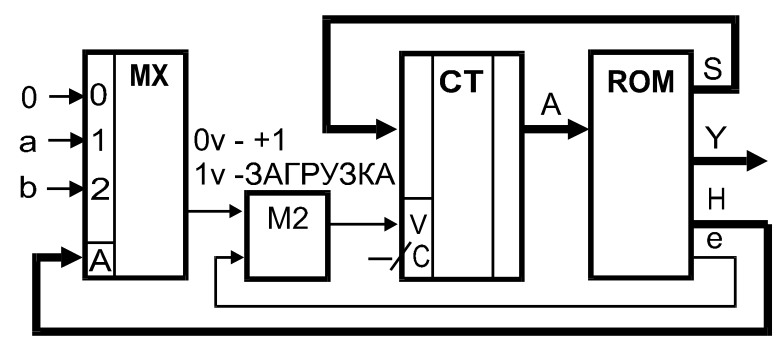
\includegraphics[width=0.5\linewidth]{regular_adress_rom}
		\caption{УА с регулярной адресацией}
		\label{img:scheme5}
	\end{center}	
\end{figure}

В конкретной реализации на информационные входы мультиплексора подаются следующие сигналы:
	\hypertarget{name}{}
\begin{itemize}

	\item Константа нуля;
	\item Ma\_IS\_NULL (признак нуля мантиссы А);
	\item Mb\_IS\_NULL (признак нуля мантиссы B);
	\item A<B (признак того, что порядок числа A меньше порядка числа B);
	\item A\_IS\_ANSWER (признак того, что ответ хранится в регистрах числа A);
	\item CT\_dP\_IS\_NULL (признак того, что счетчик разницы порядков хранит "ноль");
	\item CT\_Pa\_IS\_NULL (признак переполнения счетчика порядка числа A в большую сторону);
	\item CT\_Pa\_IS\_MAX  (признак переполнения счетчика порядка числа A в меньшую сторону);
	\item $\left|m\_a\pm m\_b\right|>1$ (признак того, что модуль алгебраической суммы операндов больше единицы);
	\item op\_normalized (признак нормализации операндов);
\end{itemize}

В схему введен элемент М2, позволяющий инвертировать значение входного сигнала, что облегчает распределение микроинструкций по ячейкам управляющей памяти.

\subsection{Алгоритм работы автомата}
Опишем алгоритм работы автомата с помощью блок схемы. См. рисунок~\ref{img:algorithm5.1} и \ref{img:algorithm5.2} в \hyperref[tam]{Приложении~А}.

После построения алгоритма работы автомата следует перейти к реализации операционной части.

\subsection {Реализация Операционного автомата}
Построим операционный автомат, выполняющий сложение двух чисел в формате с плавающей точкой. Приведем названия и назначения каждого из регистров, используемых в данном устройстве. См. таблицу \ref{tab:regs5}.
\begin{table}[h!]
	\centering
	\small
		\begin{tabular}{|m{0.27\linewidth}|m{0.6\linewidth}|}
			\hline
			\textbf{Идентификатор} & \textbf{Назначение} \\ \hline
			$RG\_Ma$ & Универсальный сдвиговый регистр. Хранит разряды мантиссы А\\ \hline
			$CT\_Mb$ & Счетчик. Хранит разряды мантиссы B\\ \hline
			$CT\_Pa$ & Счетчик. Хранит разряды порядка числа A \\\hline
			$CT\_Pb$ & Счетчик. Хранит разряды порядка числа B \\ \hline
			$CT\_dP$ & Счетчик. Хранит разряды разницы порядков чисел A и B\\ \hline
			$REG\_SUM$& Триггер. Хранит разряд сигнала переноса суммы мантисс чисел A и B\\\hline
		\end{tabular}
		\caption{Регистры операционного автомата}
		\label{tab:regs5}
\end{table}

Укажем необходимые признаки, которые впоследствии будут вырабатываться управляющим автоматом. См. таблицу \ref{tab:signals5}.
\begin{table}[h!]
	\centering
	\small
	\begin{tabular}{|m{0.17\linewidth}|m{0.7\linewidth}|}
		\hline
		\textbf{Признак} & \textbf{Назначение} \\ \hline
		$S$ & Хранит адрес следующей операции \\ \hline
		$Н$ & Адресный вход мультиплексора \\ \hline
		$R0$ & Сигнализирует об окончании операции деления \\ \hline
		$overflow$ & Сигнализирует об ошибке обработки -- переполнение \\ \hline
		$L\_Ma$ & Загрузка в регистр $RG\_Ma$ \\ \hline
		$SHIFT\_Ma$ & Правый сдвиг регистра $RG\_Ma$ если $SHIFT\_Ma\_Left=0$ и левый, если  $SHIFT\_Ma\_Left=1$ \\ \hline
		$RST$ & Асинхронный сброс всех элементов \\ \hline
		$COUNT\_Pa$ & Счет. Декремент счетчика, если $L\_CT_\_Pa==1$ \\ \hline
		$L\_CT\_Pa$ & Загрузка счетчика $CT\_Pa$ \\ \hline
		$CHANGE$ & Выбор источника загрузки в регистры мантисс и порядка чисел A и B \\ \hline
		$e$ & Управляющий сигнал для счетчика. Если $e=1$, следует выполнить загрузку, а если $e=0$ -- инкрементировать счетчик. \\ \hline
	\end{tabular}
	\caption{Осведомительные сигналы (признаки)}
	\label{tab:signals5}
\end{table}
С целью реализации левого и правого сдвига в регистре $RG\_Ma$ был построен элемент памяти, позволяющий выбрать направление сдвига с помощью двух управляющих сигналов. Данный элемент был размещен в отдельном файле и загружался в основной файл как внешняя библиотека Logisim. Устройство данного регистра можно увидеть на рисунке \ref{img:left_reg5} в \hyperref[tam]{Приложении А}.

При выполнении операции сложения предполагается, что числа, переданные на вход находятся в нормализованном виде, то есть имеют вид, представленный на сноске \ref{sign5}.

\begin{equation}
\begin{aligned}
\label{sign}
\frac12&\le \left|M\right|< 1\\
M &= 0.1XXXX\\
M &= 1.0XXXX\\
M&=1.00000\\
\end{aligned}
\end{equation}

Результат суммы также нормализуется в соответствии с данными правилами. Числа, представленные в ином виде считаются ненормализованными и не обрабатываются цифровым устройством.

Стоит отметить, что для формирования правильного выходного результата необходимо выполнить нормализацию значений суммы в зависимости от вида операндов. Для каждой комбинации операндов реализована отдельная операция нормализации. См таблицу \ref{tab:correction5}.

\begin{table}
	\small
	\begin{tabular}{|m{0.3\linewidth}|m{0.67\linewidth}|}
		\hline
		\textbf{Комбинация} &\textbf{Коррекция}\\
		\hline
		 $\left|m_a\pm m_b\right|\ge1$ & Мантисса не нормализована. Сдвинуть регистр мантиссы вправо, загрузить сигнал переноса сумматора. Увеличить порядок результата на 1. При этом может произойти переполнение счетчика в большую сторону \\ 
		\hline
		$\frac12\le \left|m_a\pm m_b\right|< 1$ & Нормализация результата не требуется\\
		\hline
		$\left|m_a\pm m_b\right|<\frac12$ & Мантисса не нормализована. Сдвигая мантиссу влево, уменьшать порядок, при этом может произойти переполнение порядка в отрицательную сторону\\
		\hline
	\end{tabular}
	\caption{Нормализация результата}
	\label{tab:correction5}
\end{table}

Соединим все элементы в соответствии с алгоритмом задачи. См. рисунки \ref{img:oa5.1} и \ref{img:oa5.2} в приложении \hyperref[tam]{Приложении А}.

\subsection {Реализация управляющего автомата}
Приступим к построению управляющего автомата, определяющего последовательность выполнения микрокоманд для сложения двух чисел в формате с плавающей точкой.

Определим разрядность ПЗУ, участвующего в построении УА по схеме с постоянной адресацией. Адрес должен иметь 5 разрядов~--- текущее значение параметра \textit{S}. Микрокоманда представлена в виде 22 бит~--- 15 признаков, расположенных в следующем порядке: S,	R0,	RST,	L\_ma,	SHIFT\_Ma,	SHIFT\_Ma\_LEFT,	L\_CT\_Pa,	COUNT\_Pa,	CHANGE,	L\_CT\_dP,	COUNT\_dP,	m\_n,	H,	e. Адрес текущей команды хранится в 5~-ти разрядном счетчике. К входам мультиплексора подлючены сигналы, значения которых анализируются в данном состоянии автомата. Они описаны выше. См. \hyperlink{name}{список}.

Заполним память в соответствии в алгоритмом, подключим ПЗУ, мультиплексор и счетчик последовательным способом. См рисунок \ref{img:ma5} в \hyperref[tam]{Приложении А}. 

Ввод и вывод результатов осуществляется с помощью блока ввода и вывода. Числа передаются в нормализованном формате со смещением порядка в С=16. См. рисунок \ref{img:inp_out5} в \hyperref[tam]{Приложении A}.


\subsection {Вывод}
В ходе данной практической работы было рассмотрено строение и работа управляющего автомата, построенного по схеме регулярной адресацией. Использовав полученные знания на практике, на основе данного управляющего автомата построено вычислительное устройство (операционный и управляющий автомат), реализующее операцию сложения двух чисел в формате с плавающей точкой.

\newpage{
\centering
\anonsection{ПРИЛОЖЕНИЕ А}
}
\label{tam}

% 3 работа
\begin{figure}[h!]	
	\centering
	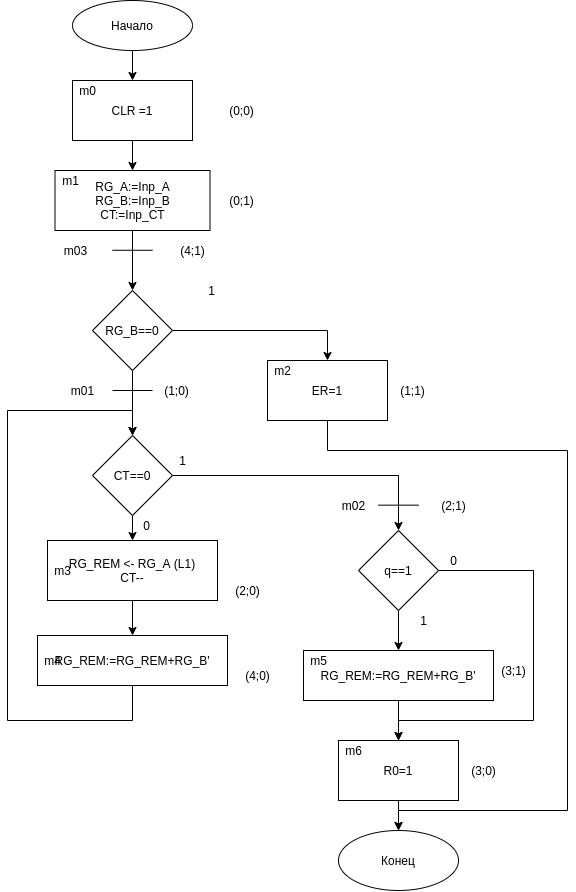
\includegraphics[width=0.6\linewidth]{algorithm3}
	\caption {Алгоритм деления двух 4-разрядных чисел}
	\label{img:algorithm3}
\end{figure}
\newpage
\begin{figure}[h!]
	\centering
	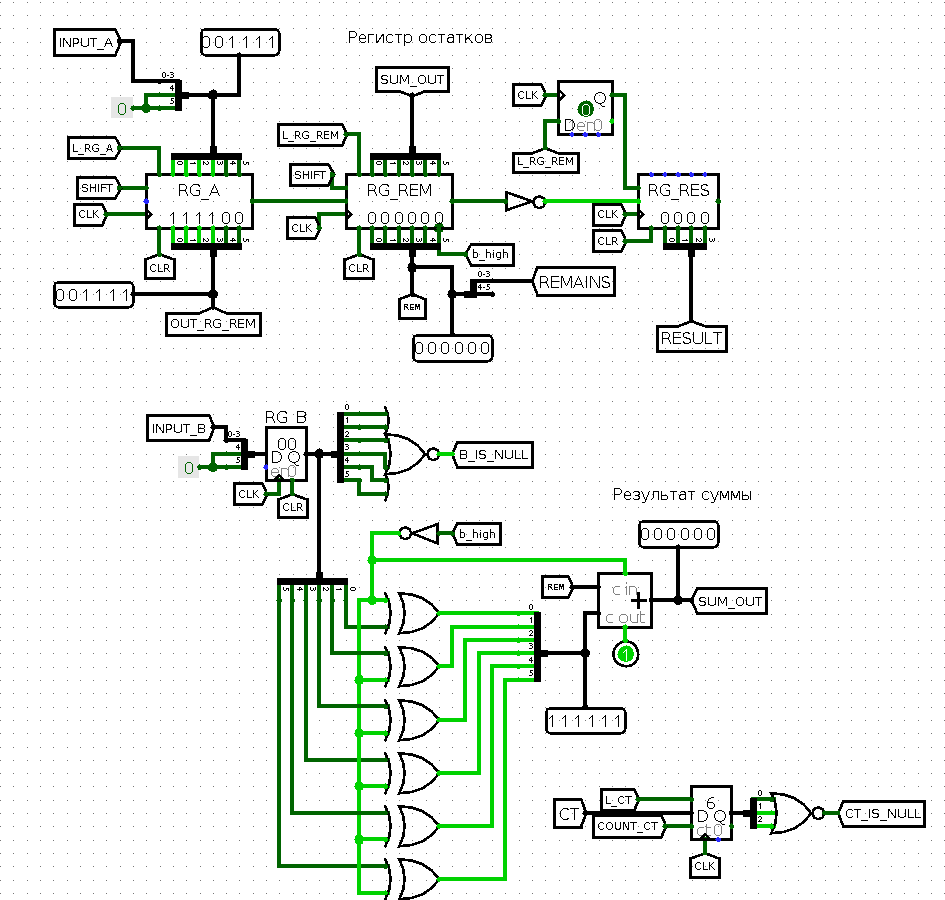
\includegraphics[width=0.5\linewidth]{OA3}
	\caption {Схема операционного автомата}
	\label{img:oa3}
\end{figure}

% 4 работа


\begin{figure}[h!]
	\centering
	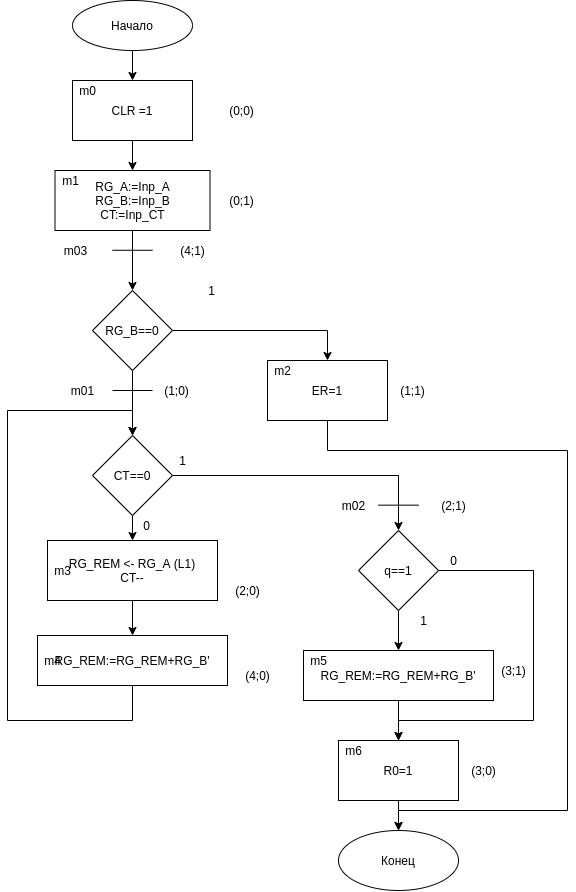
\includegraphics[width=0.5\linewidth]{algorithm3}
	\caption {Алгоритм деления двух 4-разрядных чисел}
	\label{img:algorithm4}
\end{figure}
\newpage
\begin{figure}[htpb]
	\centering
	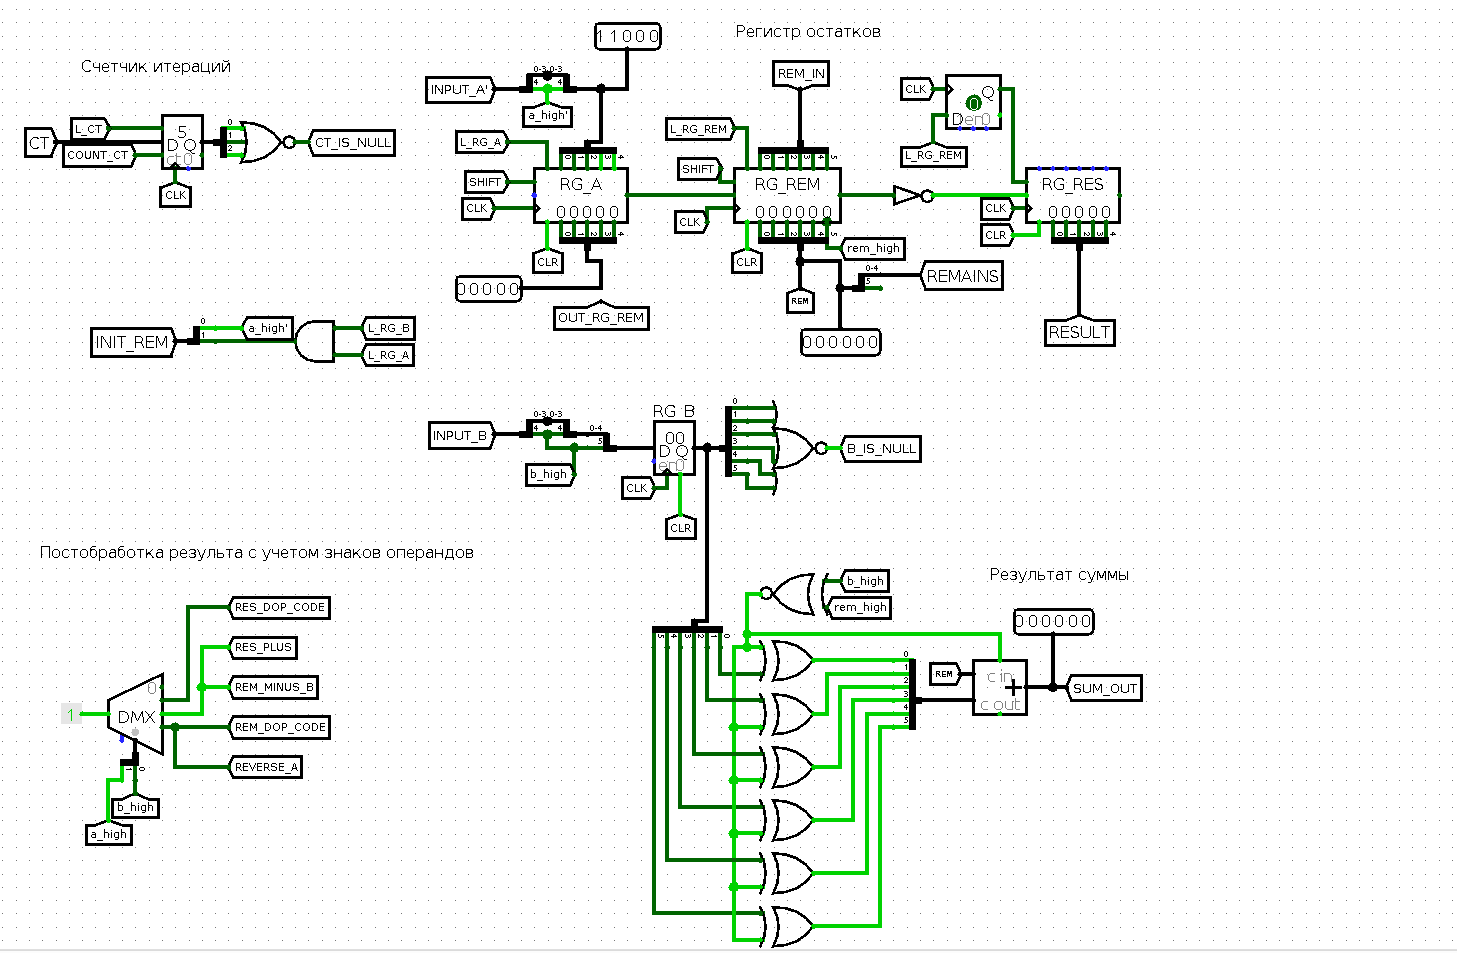
\includegraphics[width=0.6\linewidth]{OA4.1}
	\caption {Схема операционного автомата, часть 1}
	\label{img:oa4.1}
\end{figure}
\begin{figure}[htpb]
	\centering
	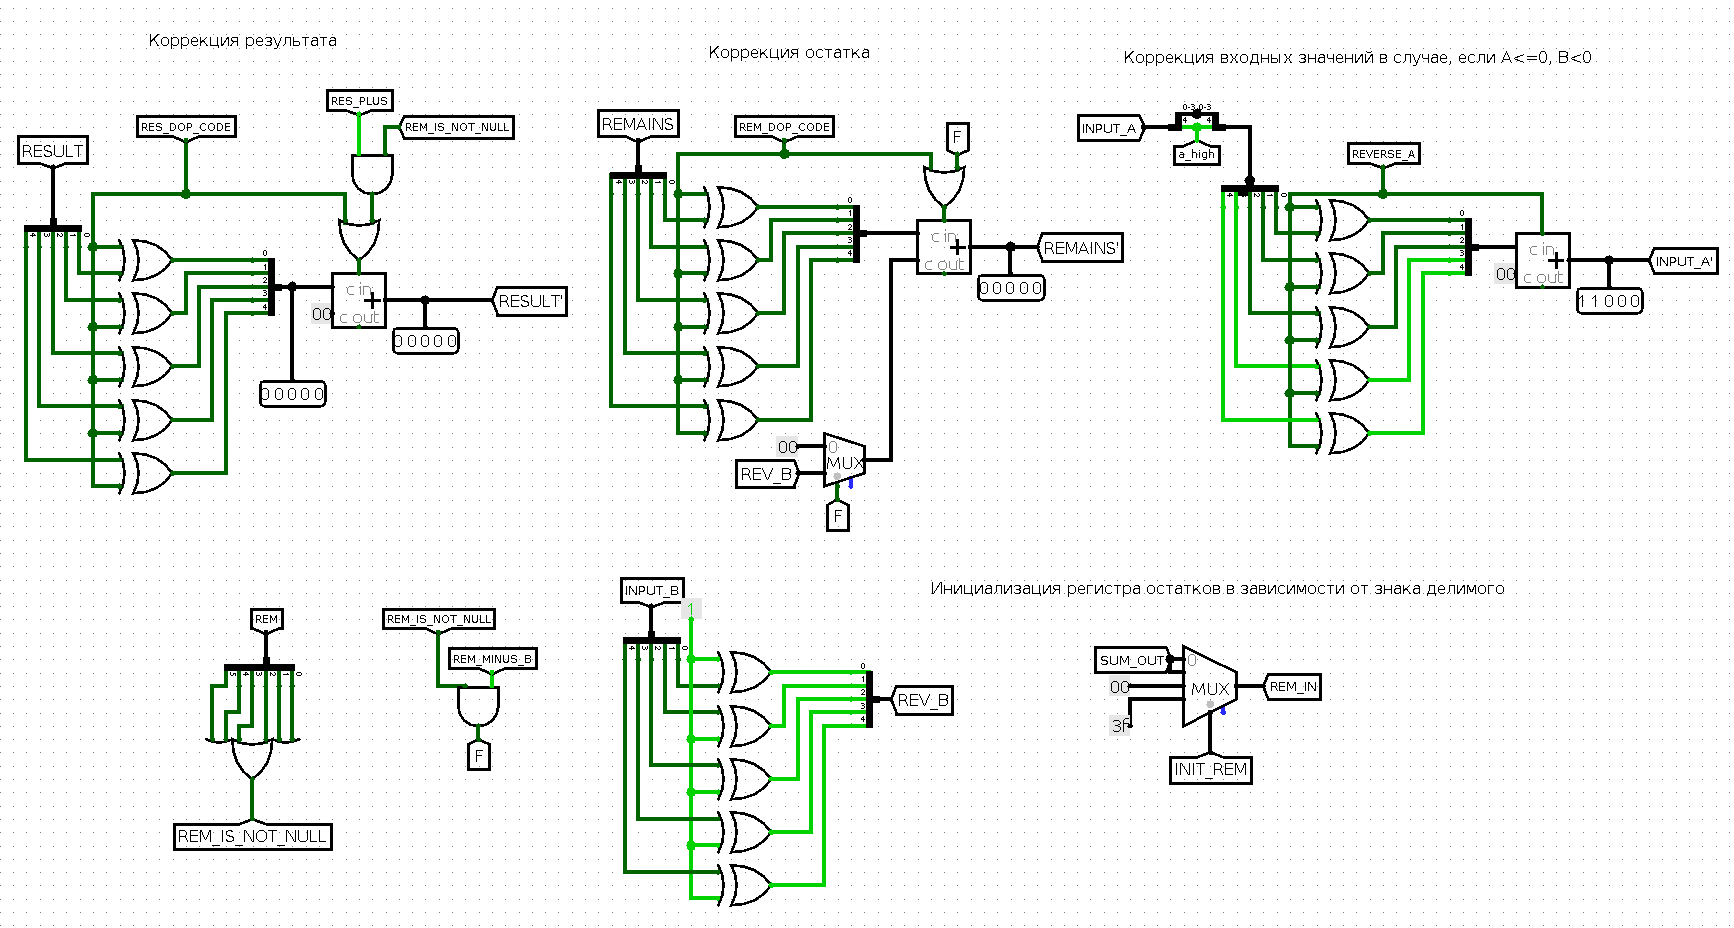
\includegraphics[width=0.6\linewidth]{OA4.2}
	\caption {Схема операционного автомата, часть 2}
	\label{img:oa4.2}
\end{figure}

\begin{figure}[h!]
	\centering
	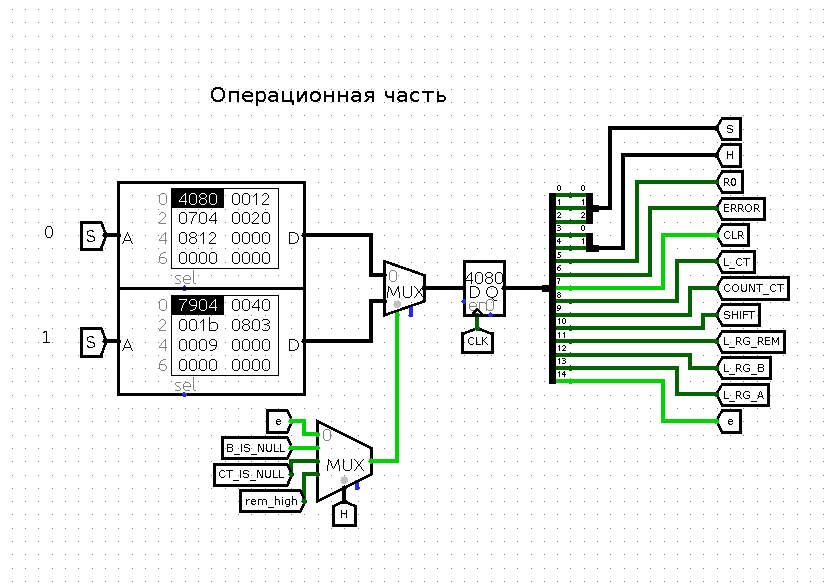
\includegraphics[width=0.6\linewidth]{MA4}
	\caption {Схема операционного автомата}
	\label{img:ma4}
\end{figure}

% 5 работа
\newpage
\begin{figure}[h!]
	\centering
	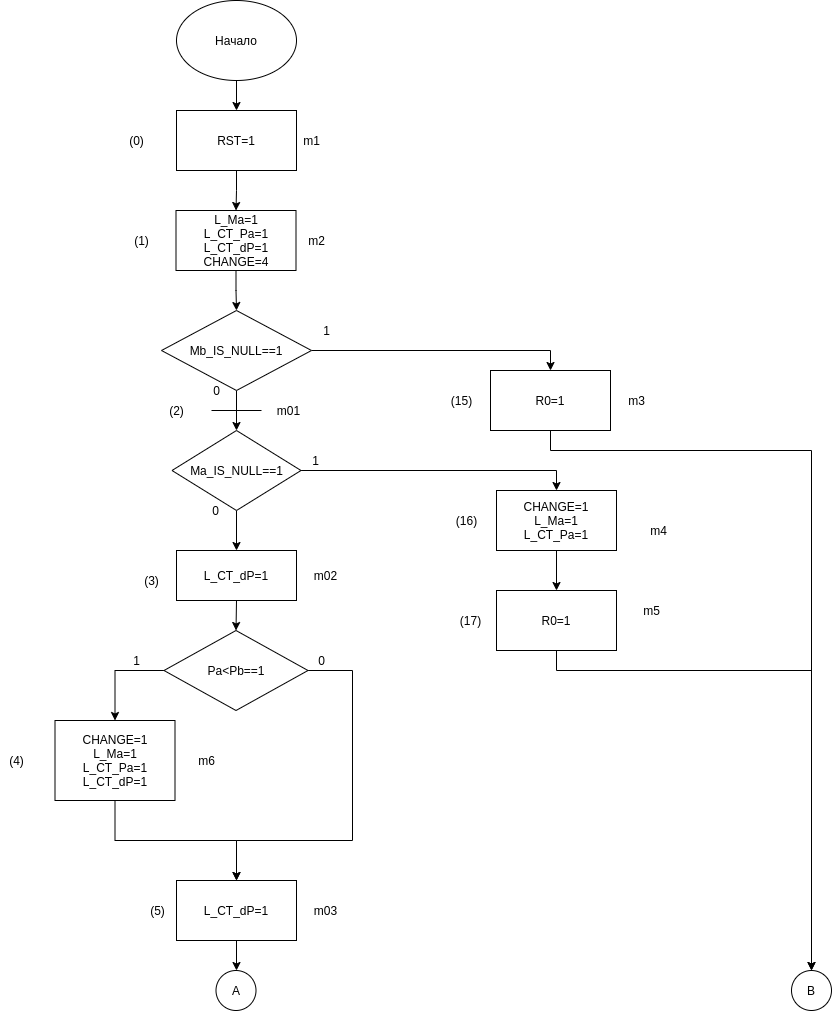
\includegraphics[width=0.3\linewidth]{algorithm5.1}
	%\caption {Алгоритм сложения чисел с плавающей точкой. Часть 1}
	\label{img:algorithm5.1}
\end{figure}
%\newpage
\begin{figure}[h!]
	\centering
	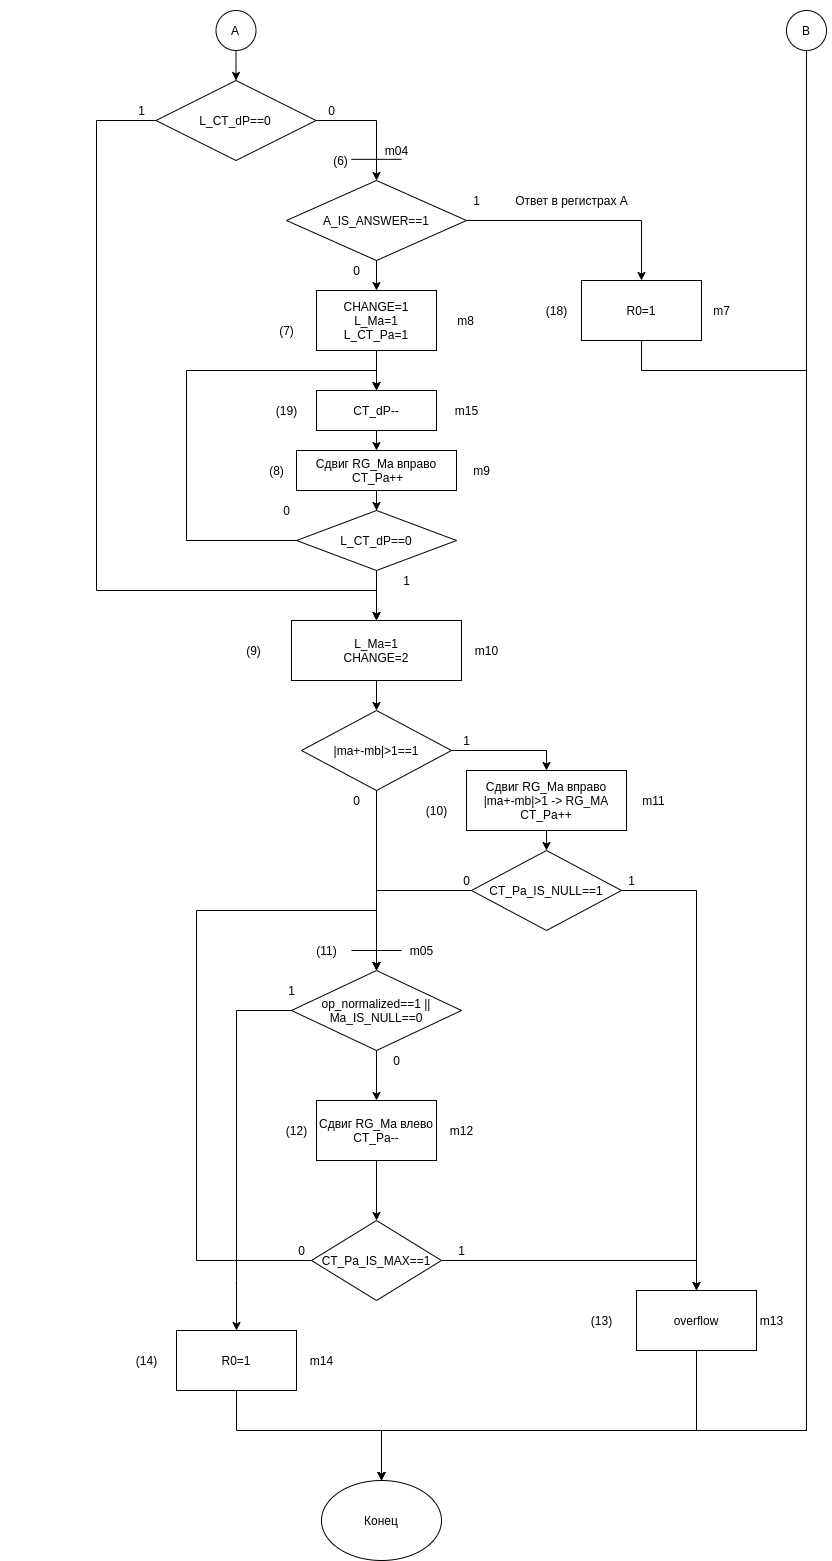
\includegraphics[width=0.4\linewidth]{algorithm5.2}
	\caption {Алгоритм сложения чисел с плавающей точкой. Часть 2}
	\label{img:algorithm5.2}
\end{figure}
\newpage
\begin{figure}[h!]
	\centering
	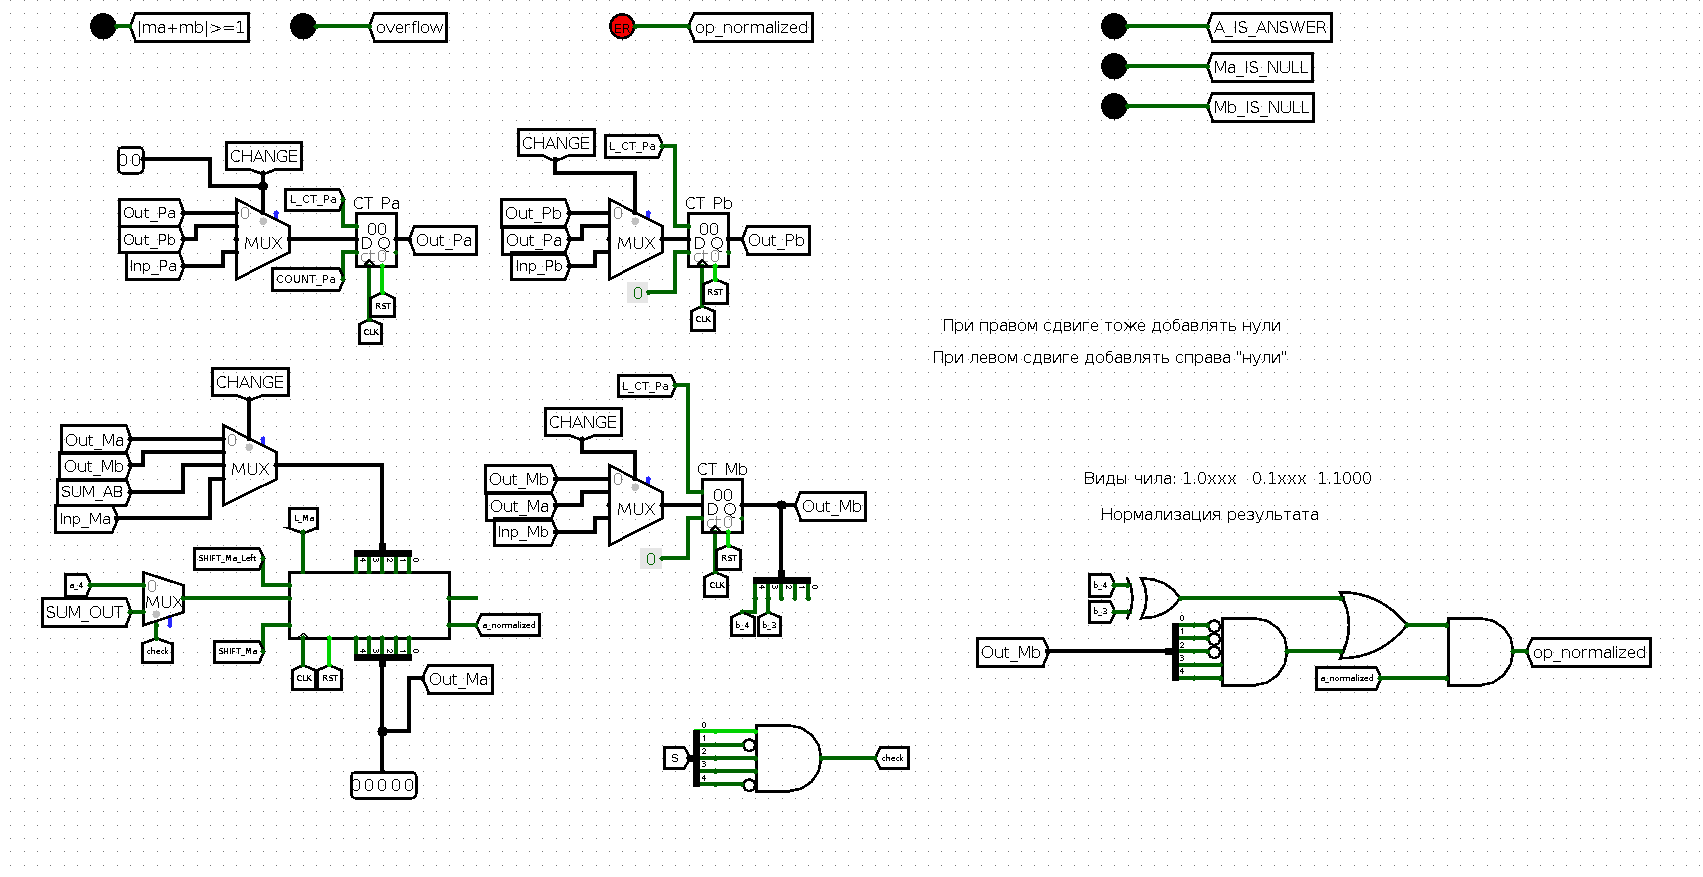
\includegraphics[width=0.6\linewidth]{oa5.1}
	\caption {Схема операционного автомата, часть 1}
	\label{img:oa5.1}
\end{figure}
\begin{figure}[h!]
	\centering
	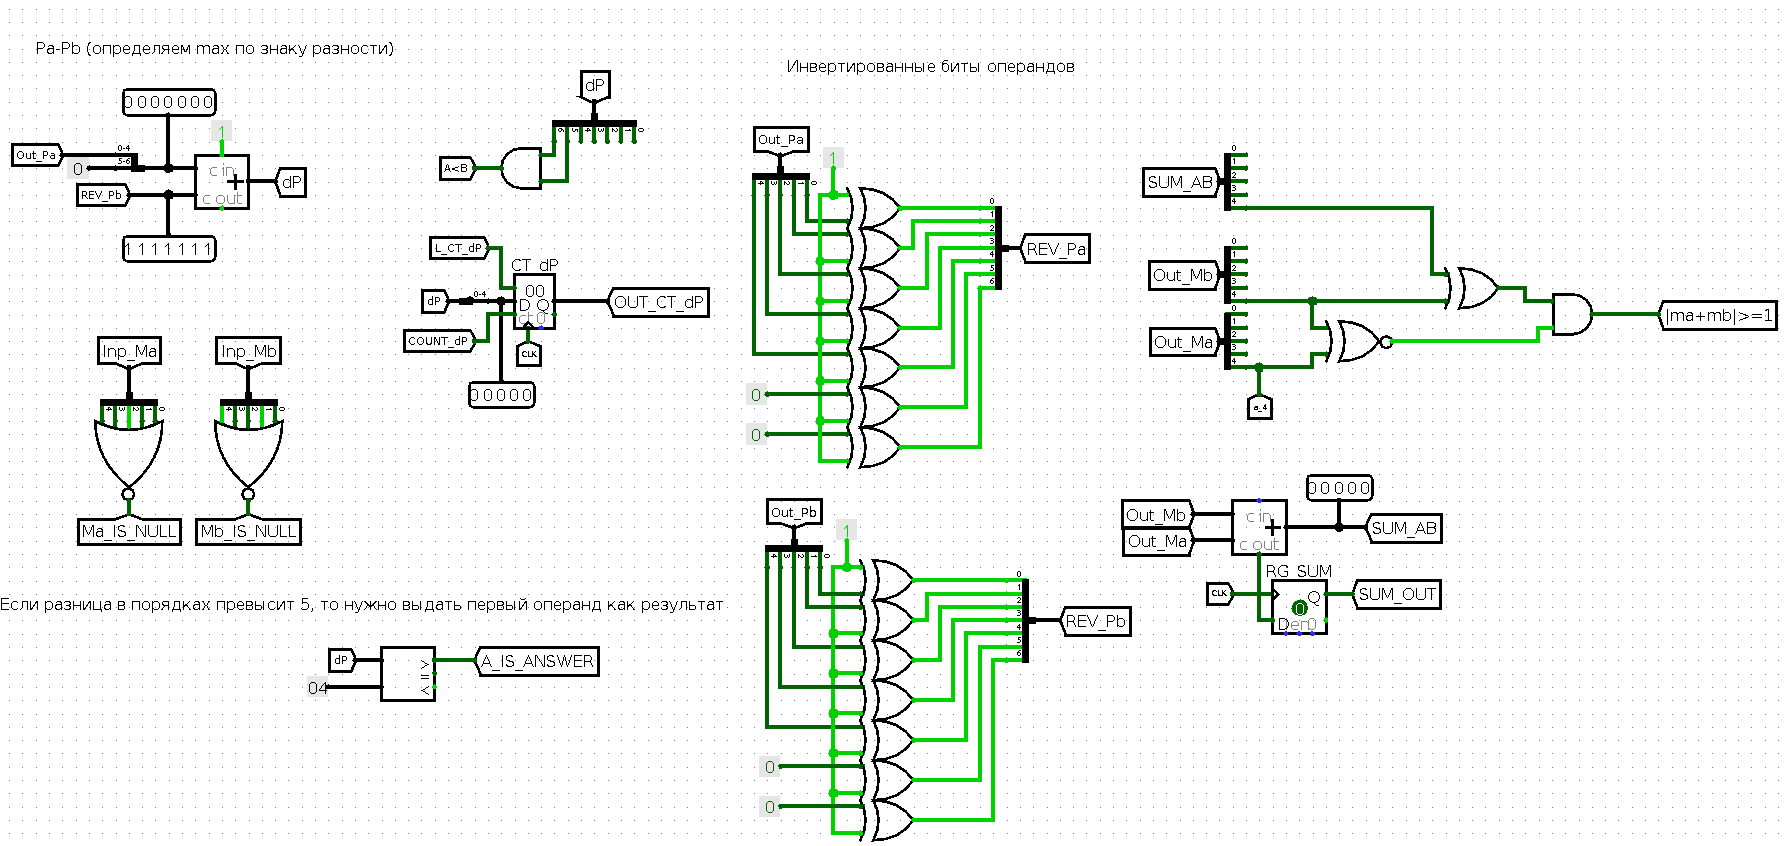
\includegraphics[width=0.6\linewidth]{oa5.2}
	\caption {Схема операционного автомата, часть 2}
	\label{img:oa5.2}
\end{figure}

\begin{figure}[h!]
	\centering
	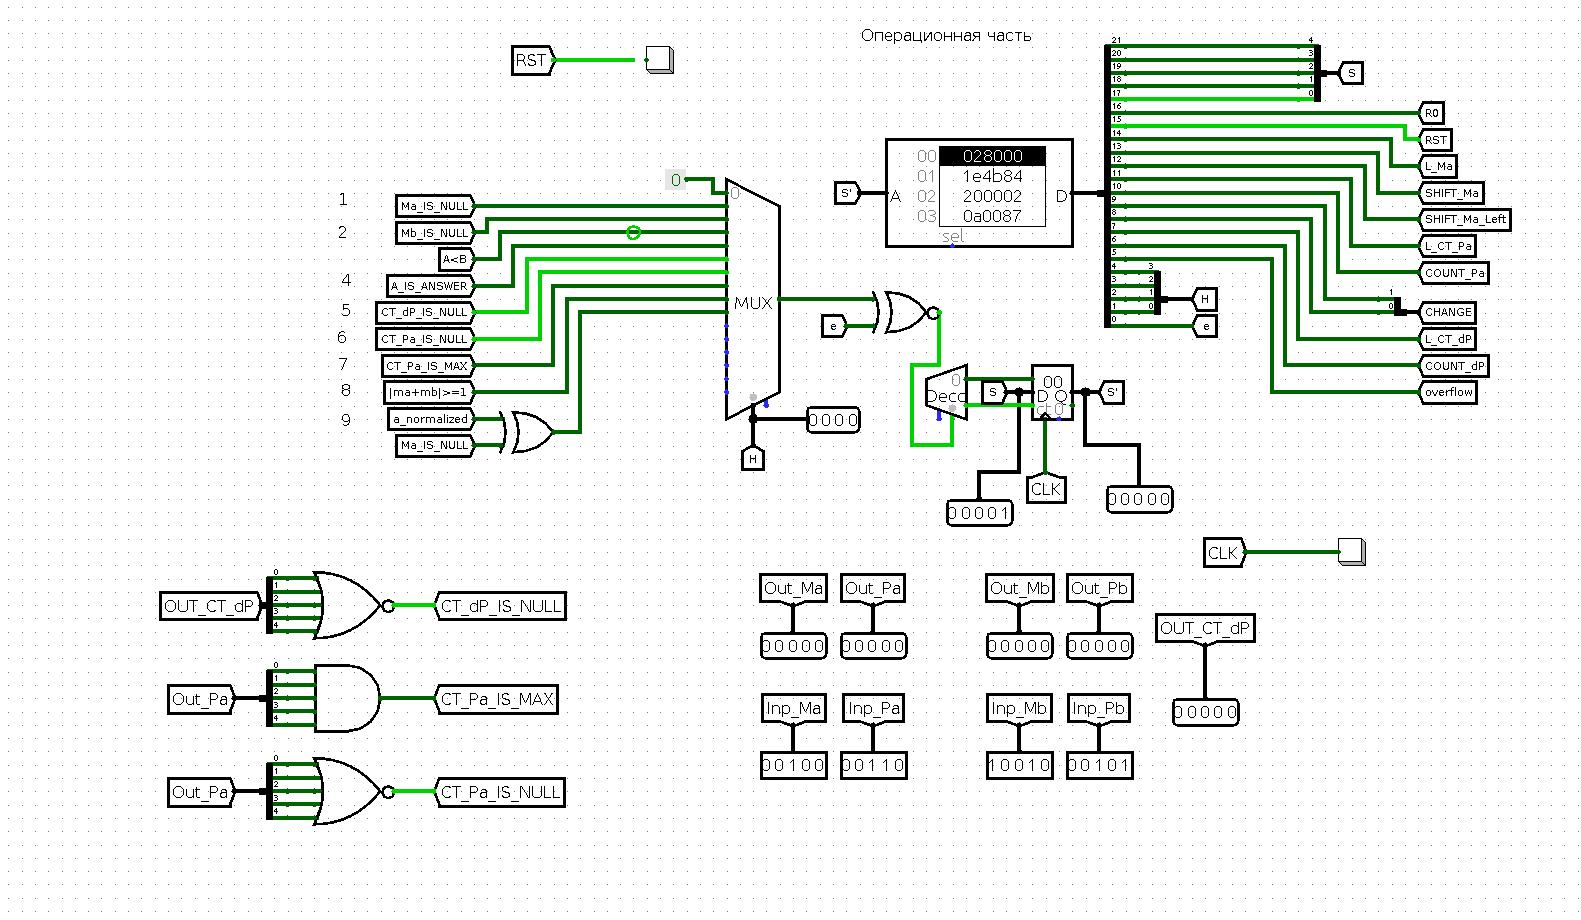
\includegraphics[width=0.6\linewidth]{ma5}
	\caption {Схема управляющего автомата}
	\label{img:ma5}
\end{figure}
\newpage
\begin{figure}[h!]
	\centering
	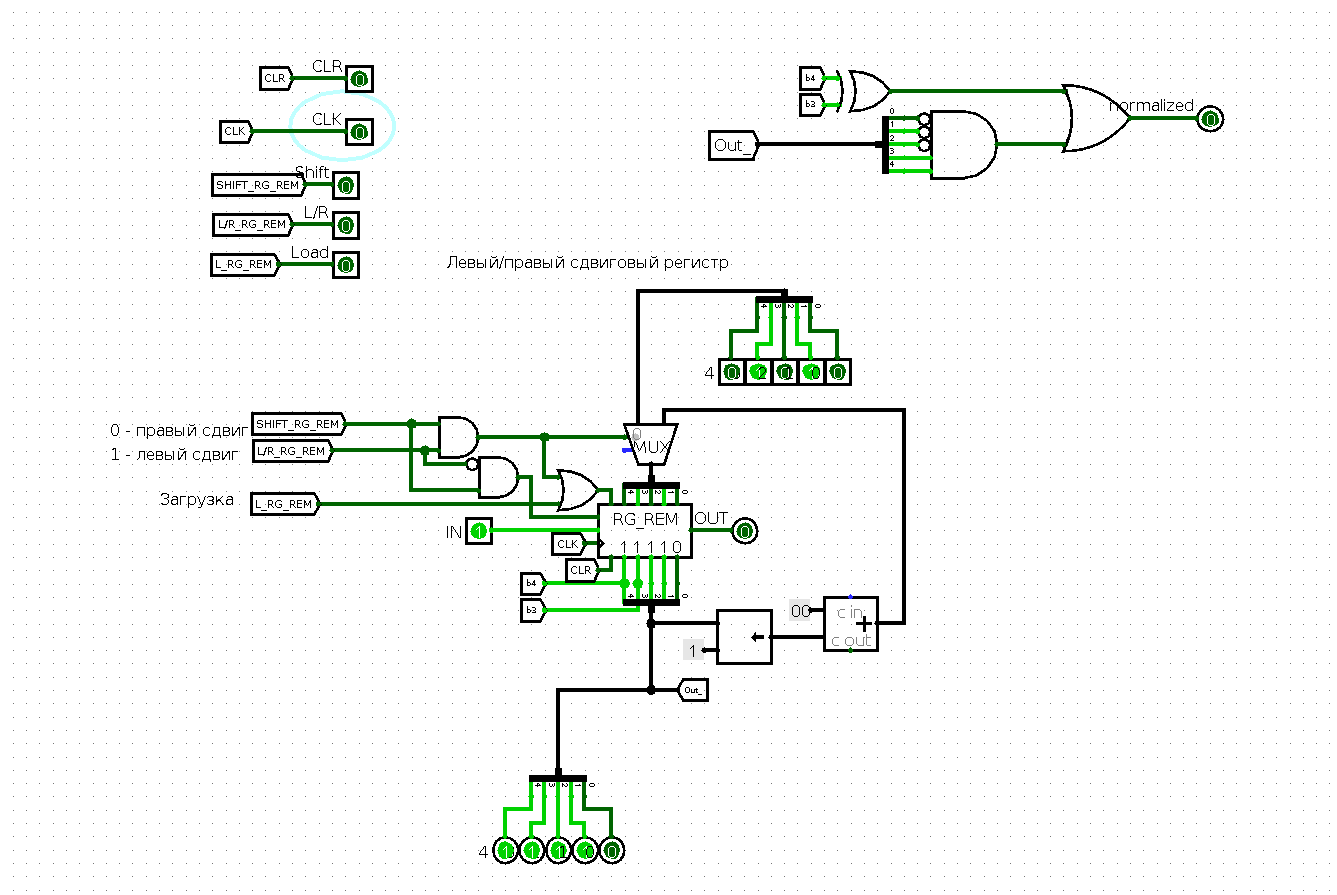
\includegraphics[width=0.6\linewidth]{left_reg}
	\caption {Устройство универсального регистра}
	\label{img:left_reg5}
\end{figure}

\begin{figure}[h!]
	\centering
	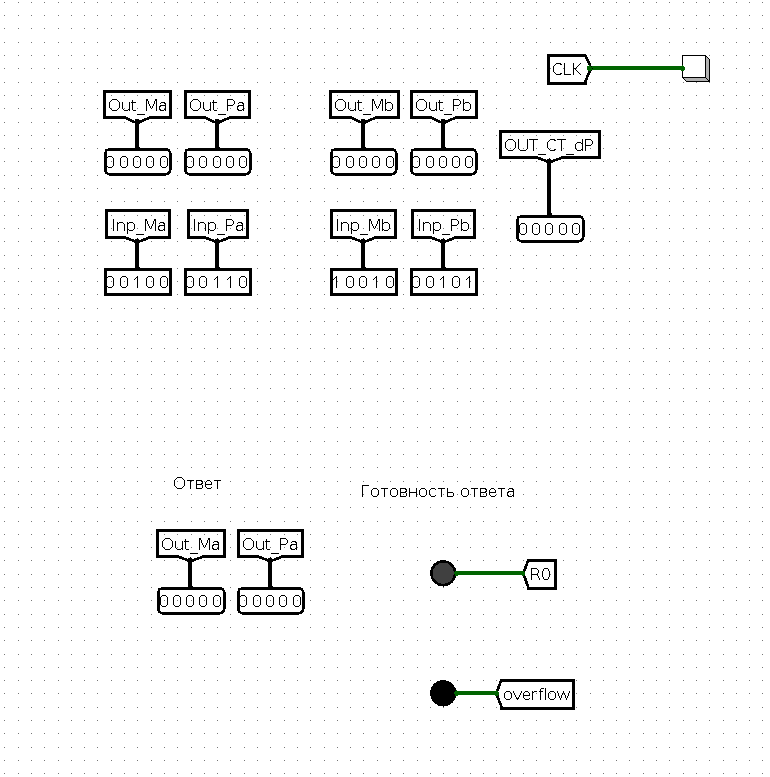
\includegraphics[width=0.6\linewidth]{inp_out}
	\caption {Блок ввода-вывода}
	\label{img:inp_out5}
\end{figure}

\end{document}


